\documentclass[12pt,oneside]{report}
\usepackage{amsmath} % \usepackage is a command that allows you to add functionality to your LaTeX code
\usepackage[papersize={215mm,280mm},tmargin=25mm,bmargin=25mm,lmargin=25mm,rmargin=25mm]{geometry}

\usepackage[english]{babel}
\usepackage[utf8]{inputenc}

\usepackage{amsmath,amssymb,mathabx,amsthm}%\for eqref
\usepackage{mathabx}
\usepackage{lscape}
\usepackage{graphicx}
\usepackage{tikz}\usetikzlibrary{arrows.meta,calc} %library tikz
\usepackage{subcaption}
\usepackage[labelfont=bf]{caption}
\usepackage{float}
\usepackage{pgfplots}
\pgfplotsset{compat=1.15}
\usepackage{mathrsfs}
\usetikzlibrary{arrows}
\usepackage{pstricks}
\usepackage{multido}
\usepackage{pst-plot}
\usepackage{rank-2-roots}


\usepackage{color,soul} %package for highlining
\usepackage[colorinlistoftodos]{todonotes}
\usepackage{fancyhdr}
\usepackage{hyperref} %creat hyperlink
\hypersetup{
    colorlinks=true,
    linkcolor=blue,
    filecolor=magenta,      
    urlcolor=cyan,
    pdftitle={Overleaf Example},
    pdfpagemode=FullScreen,
    } %set up a hyperlink to be in blue 
\newtheorem{definition}{Definition}[section]
\newtheorem{theorem}[definition]{Theorem}
\newtheorem{prop}[definition]{Proposition}
\newtheorem{lemma}[definition]{Lemma}
\newtheorem{example}[definition]{Example}

\newtheorem*{remark}{Remark}
\lhead{}%clear the lead head
\linespread{1.25}



\pagestyle{fancy}
\cfoot{\thepage} % this is for the page numbering
\setlength\parindent{0pt} % noindent for the whole document.
 % increase the distance between line.

    
\DeclareMathOperator{\SLn}{\text{SL}_n(\mathbb{R})}
\DeclareMathOperator{\GLn}{\text{GL}_n(\mathbb{R})}
\DeclareMathOperator{\glnr}{\mathfrak{gl}_n(\mathbb{R})}
\DeclareMathOperator{\slnz}{SL_n(\mathbb{Z})}
\DeclareMathOperator{\glnz}{GL_n(\mathbb{Z})}
\DeclareMathOperator{\vol}{vol}
\DeclareMathOperator{\rk}{rank}
\DeclareMathOperator{\Hom}{Hom}
\DeclareMathOperator{\fg}{\mathfrak{g}}
\DeclareMathOperator{\fh}{\mathfrak{h}}
\DeclareMathOperator{\SOn}{SO_n(\mathbb{R})}
\DeclareMathOperator{\On}{O_n(\mathbb{R})}
\DeclareMathOperator{\slnr}{\mathfrak{sl}_n(\mathbb{R})}
\DeclareMathOperator{\Ad}{\text{Ad}}
\DeclareMathOperator{\SLR}{SL_2(\mathbb{R})}
\DeclareMathOperator{\slz}{SL_2(\mathbb{Z})}
\DeclareMathOperator{\sl2}{\mathfrak{sl}_2(\mathbb{R})}
\DeclareMathOperator{\SO2}{SO_2(\mathbb{R})}
\DeclareMathOperator{\uH}{\mathfrak{H}}
\DeclareMathOperator{\cpx}{\textbf{cp}(x)}


\begin{document}
% uncomment this line when submitting to Library and Archives Canada,
% as they need a single-sided version.
\setboolean{@twoside}{true}

\flushbottom
\thispagestyle{empty}
%%%%%%%%%%%%%%%%%%%%%%%%%%%%%%%%%%%%%%%%%%%%%%%%%%%%%%%%%%%%%%%%%%%
%%%%%%%%%%%%%%%%%%%%%%%%%%%%%%%%%%%%%%%%%%%%%%%%%%%%%%%%%%%%%%%%%%%
%%%%%%%%%%%%%%%%%%%%%%%%%%%%%%%%%%%%%%%%%%%%%%%%%%%%%%%%%%%%%%%%%%%
% this sets the metadata for the PDF (if compiled with pdflatex)
% FILL THIS IN!!!
\def\ThesisTitle{On Semi-stable lattices in higher rank}
\def\ThesisAuthor{Nguyen Pham Minh Tri}
% convocation date must either be ``Spring 20xx'' or ``Fall 20xx''
\convocationdate{Summer 2026}
%\degree{Doctor of Philosophy}
\degree{Masters of Science}

\supervisor{Dr.\ Supervisor}
%\cosupervisor{your co-supervisor} % if applicable
\firstcommitteemember{Dr.\ Committee Person}
\secondcommitteemember{Dr.\ Committee Person}
%\thirdcommitteemember{}
%\fourthcommitteemember{}
%\fifthcommitteemember{}

\department{Department of Mathematical and Statistical Sciences}
% If you have a specialization, enter it here
\fieldofstudy{Mathematics}
%%%%%%%%%%%%%%%%%%%%%%%%%%%%%%%%%%%%%%%%%%%%%%%%%%%%%%%%%%%%%%%%%%%
%%%%%%%%%%%%%%%%%%%%%%%%%%%%%%%%%%%%%%%%%%%%%%%%%%%%%%%%%%%%%%%%%%%
%%%%%%%%%%%%%%%%%%%%%%%%%%%%%%%%%%%%%%%%%%%%%%%%%%%%%%%%%%%%%%%%%%%


\definecolor{heavyblue}{cmyk}{1,1,0,0.25}
\hypersetup{
  pdftitle=\ThesisTitle,
  pdfauthor=\ThesisAuthor,
  pdfpagemode=UseOutlines,
  citebordercolor=0 0 1,
  colorlinks=true,
  allcolors=heavyblue,
  breaklinks=true,
  pdfpagetransition=Dissolve,
  bookmarks=true
}
\title{\ThesisTitle}
\author{\ThesisAuthor}

\beforebodyoftex

\titlepage

\newpage\setcounter{page}{0}\thispagestyle{empty}$\text{ }$
\newpage\setcounter{page}{2}

%\libraryreleaseform %%% not currently required by FGSR
%\signaturepage %%% not currently required by FGSR

%\begin{dedication}
% put your dedication here
%\end{dedication}


\begin{abstract}
\doublespacing
 In this thesis, we study the notion of semi-stable lattices in two dimensional space and generalize it to finite dimensional space of dimension at least 3.

 The semi-stable lattices can be defined using two different definition, as first defined using a plot as in \cite{MR780079} and later defined using Harish-Chandra map as in \cite{MR3969872}. We showed that 
 the two definition are equivalent and proved the equivalence between geometric properties using plot and algebraic properties using Harish-Chandra map. We achieve this by pointing out the volume of sublattices can be computed 
 using pairing between Harish-Chandra map with the Weyl vectors. In this way, the geometric information and algebraic information are the same.
 
 When the lattice is not semi-stable, which is called unstable, it can be attached 
 a canonical plot in geometric sense and a  canonical pair in algebraic sense. We also proved that these objects encode essentially the same data in finite dimensional case. 
\end{abstract}
\newpage
\tableofcontents
\newpage
\listoffigures
\newpage
\begin{preface}
This thesis is an original work by Tri Nguyen. No part of this thesis has been previously published. 
\end{preface}

\addcontentsline{toc}{chapter}{Preface}

\pagenumbering{arabic}

\chapter{$\SLR$} % Sets article title

In this chapter, I will give an exposition on the structure of $\SLR$ as the spaces of lattice, this space
plays the role of a toy model before exploring the space of lattice in the higher rank. The exposition follows
the paper \cite{} and  \cite{} closely.
\section{$\SLR$ and its action on the upper half plane $\uH$}
A priori, the upper half plane
\[\uH = \left\lbrace z: \Im z >0 \right\rbrace \subset \mathbb{C}\]
has no group structure on its. However, we will show below that it can identify topologically with the space
with the space of cosets $\SO22\backslash\SLR$, and thus we can study the spaces $\uH$ via the spac of lattices $\SO2\backslash\SLR$.
We define the action of $G= \SLR$ on $\uH$ as follows
\[
  \begin{bmatrix}a & b \\ c & d\end{bmatrix} \circ (z) = \frac{dz -b}{-cz + a}
\]
\begin{prop}\label{h-as-matrices}
  The group $\SLR$ stabilizes \(\mathfrak{H}\) and acts transitively on it. In particular,
  \[
    \begin{bmatrix}\frac{1}{\sqrt{y}} & 0 \\ 0 & \sqrt{y}\end{bmatrix}\begin{bmatrix}1 & -x \\ 0 & 1\end{bmatrix}(i) = x + iy \quad (\text{for } x \in \mathbb{R}, \, y > 0)
  \]
  Further, for \(g = \begin{bmatrix}a & b \\ c & d\end{bmatrix} \in SL_{2}(\mathbb{R})\) and \(z \in \mathfrak{H}\),
  \[
    \text{$\Im$}\,g(z) = \frac{\text{$\Im$}\,z}{|cz + d|^2}.
  \]
\end{prop}
\begin{proof}
  The first formula is clear. The second formula would imply that the upper half-plane is stabilized. Compute directly:
  \[
    2i \cdot \text{$\Im$} \left( \begin{bmatrix} d & -b \\ -c & a \end{bmatrix} \circ(z) \right) = \frac{az + b}{cz + d} - \frac{d\overline{z} + b}{c\overline{z} + d} = \frac{(az + b)(c\overline{z} + d) - (a\overline{z} + b)(cz + d)}{|cz + d|^2}
  \]
  \[
    = \frac{adz - bc\overline{z} - bcz + ad\overline{z}}{|cz + d|^2} = \frac{z - \overline{z}}{|cz + d|^2}
  \]
  since \( ad - bc = 1 \).
\end{proof}
The point $z = i$ is special, in the sense that its stability group is the orthogonal group $K =\SO2$. Indeed, for any \(g = \begin{bmatrix}d & -b \\ -c & a\end{bmatrix} \in SL_{2}(\mathbb{R})\)  we have
that
\[g \circ i = i \Leftrightarrow \dfrac{ai+b}{ci+d }=i \Leftrightarrow a=d \text{ and } b = -c \]
Combinining with the fact that $ad-bc=1$, we must have $a^2 + b^2=1$. This implies that there is a $\theta$ such that $a = \cos\theta$ and $b = \sin \theta$.
Since $G$ acts on $\uH$ transitively, we know from group theory that there is a bijection between the collection of cosets of
$\text{Stab}(i)$ in $G$ and the orbits of $i$. In particular
\begin{prop}\label{upper-group}
  We have an isomorphism of \(SL_{2}(\mathbb{R})\)-spaces
  \[
    \SO2\backslash\SLR \cong \mathfrak{H} \quad \text{via} \quad  SO(2)g \to g^{-1}(i)
  \]
  That is, the map respects the action of \(\text{SL}_{2}(\mathbb{R})\), in the sense that
  \[
    (\SO2 g)\cdot h \;\longrightarrow\; h^{-1}(g^{-1}i)
  \]
\end{prop}
\begin{proof}
  This is because of \textit{associativity}:
  \[
    (\SO2 g)\cdot h  = (\SO2)\cdot (gh)  \;\longrightarrow\; (gh)^{-1}(i) = h^{-1}(g^{-1}(i))
  \]
  giving the result.
\end{proof}
\section{Fundamental domain for $\Gamma = SL_2(\mathbb{Z})$ on $\mathfrak{H}$}
Here is a picture of the fundamental domain $\mathfrak{H}/\Gamma$.
\[
  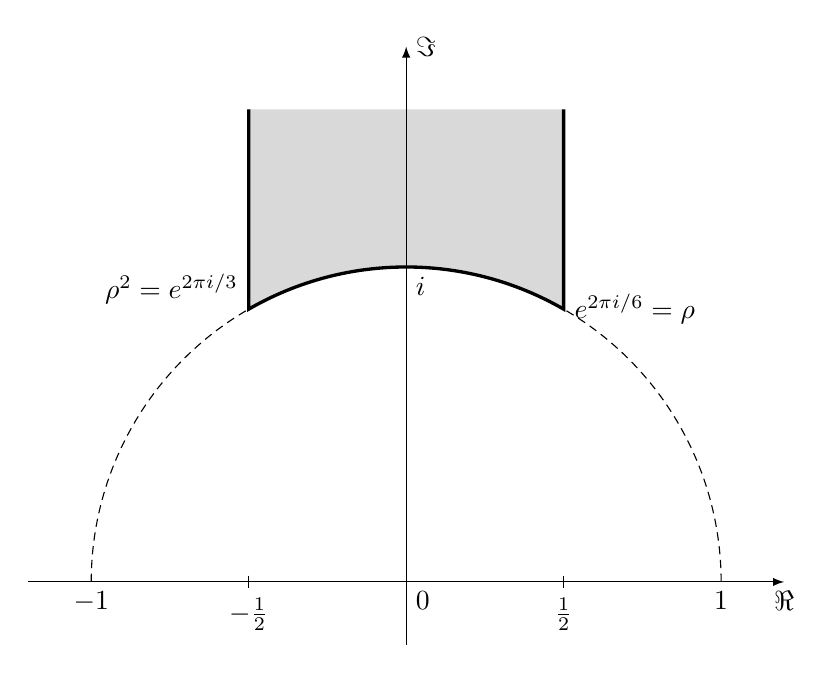
\begin{tikzpicture}[scale=4]
    \draw[densely dashed] (1,0) arc (0:60:1) (-1,0) arc (180:120:1);
    \draw[very thick, fill=gray!30] (.5,1.5) --node[right, pos=1]{$e^{2\pi i/6}=\rho$} (60:1) arc (60:120:1)
    --node[left, pos=.1]{$\rho^2=e^{2\pi i/3}$} (-.5,1.5);
    \draw[-latex] (-1.2,0) -- (1.2,0)node[below]{$\Re$};
    \draw[-latex] (0,-.2) -- (0,1.7)node[right]{$\Im$};
    \path(-1,0) --node[below, pos=0]{$-1$}node[below right, pos=.5]{0}node[below, pos=1]{1} (1,0)
    (0,1)node[below right]{$i$};
    \draw(-.5,.02)--(-.5,-.02)node[below]{$-\frac{1}{2}$}(.5,.02)--(.5,-.02)node[below]{$\frac{1}{2}$};
  \end{tikzpicture}\]
The goal of this section is to prove that under the action of the $\Gamma = \slz$, we can "move"
every points on the upper half plane to a domain, under an equivalence given by a specific action.
This is similar to the fundamental domain given by the translation action of $\mathbb{Z}$ to $\mathbb{R}$ is the half-open
unit interval $[0,1)$. In general, this give a simpler description to the homogenous space of lattice.

Note that when we try to compute the fundamental domain of $\mathbb{Z}\backslash \mathbb{R}$, we have $\mathbb{Z}$ plays a role of
\textit{discrete} subset of $\mathbb{R}$. We give a precise definition of discreteness as follows
\begin{definition}
  Let a group $G$ act continuously on a topological space $X$. A subset $\Gamma \subset G$ is called \textbf{discrete} if for any two compact subse
  $A,B$ in $X$, there are only finitely many $g \in \Gamma$ such that $g \circ A \cap B \ne \emptyset$.
\end{definition}
We will prove that the set
\[\Gamma = \slz = \left\lbrace \begin{bmatrix}
    a & b \\
    c & d
  \end{bmatrix} \in \SLR: a, b, c, d \in \mathbb{Z}\right\rbrace\]
is a discrete subgroup of $G = \SLR$.
To prove this, we first need the following lemma
\begin{lemma}\label{lm2}
  Fix a real number $r>0$ and $0<\delta<1$. We denote $R_{r,\delta}$ the rectangle
  \[R_{r,\delta} = \left\lbrace z = x+iy: -r \le x \le r, 0 <\delta \le y \le \delta^{-1}\right\rbrace\]
  Then for any $\epsilon >0$ and any fixed set $\mathbb{S}$ of coset representatives for $\Gamma_\infty\backslash \Gamma$, there are finitely
  many $g \in \mathbb{S}$ such that $\Im(g\circ z)>\epsilon$ for some $z \in R_{r,\delta}$.
\end{lemma}
In the above lemma, the notation $\Gamma_\infty$ is defined to be the set
\[ \Gamma_\infty = \left\lbrace\begin{bmatrix}
    1 & n \\
    0 & 1
  \end{bmatrix}: n \in \mathbb{Z} \right\rbrace.\] It can be seen easily that this is the
stability group of $\infty$ in $\mathfrak{H}$.
\begin{proof}
  Let \( g = \begin{bmatrix} d & -b \\ -c & a \end{bmatrix} \). Then for \( z \in R_{r, \delta} \),
  \[
    \text{Im}(g \circ z) = \frac{y}{c^2 y^2 + (cx + d)^2} < \epsilon
  \]
  if \( |c| > (y \epsilon)^{-\frac{1}{2}} \). On the other hand, for \( |c| \leq (y \epsilon)^{-\frac{1}{2}} \leq (\delta \epsilon)^{-\frac{1}{2}} \), we have
  \[
    \frac{y}{(cx + d)^2} < \epsilon
  \]
  if the following inequalities hold:
  \[
    |d| > |c| r + (y \epsilon^{-1})^{\frac{1}{2}} \geq |c| r + (\epsilon \delta)^{-\frac{1}{2}}.
  \]
  Consequently, \(\Im(g \circ z) > \epsilon\) only if
  \[
    |c| \leq (\delta \epsilon)^{-\frac{1}{2}} \quad \text{and} \quad |d| \leq (\epsilon \delta)^{-\frac{1}{2}} (r + 1),
  \]
  and the total number of such pairs (not counting $(c, d) = (0, \pm 1), (\pm 1, 0)$) is at most $\frac{4(r+1)} {(\epsilon \delta)}$. This proves the lemma.
\end{proof}
It follows from Lemma \ref{lm2} that $\Gamma = \text{SL}(2, \mathbb{Z})$ is a discrete subgroup of $SL(2, \mathbb{R})$. This is because:

\begin{enumerate}
  \item It is enough to show that for any compact subset $A \subset \mathfrak{H}$ there are only finitely many $g \in SL(2, \mathbb{Z})$ such that $(g \circ A) \cap A \neq \phi$;

  \item Every compact subset of $A \subset \mathfrak{H}$ is contained in a rectangle $R_{r,\delta}$ for some $r > 0$ and $0 < \delta < \delta^{-1}$;

  \item $((\alpha g) \circ R_{r,\delta}) \cap R_{r,\delta} = \phi$, except for finitely many $\alpha \in \Gamma_{\infty}$, $g \in \Gamma_{\infty}\backslash \Gamma$.
\end{enumerate}

To prove (3), note that Lemma \ref{lm2} implies that $(g \circ R_{r,\delta}) \cap R_{r,\delta} = \phi$ except for finitely many $g \in \Gamma_{\infty}\backslash \Gamma$. Let $S \subset \Gamma_{\infty}\backslash \Gamma$ denote this finite set of such elements $g$. If $g \not\in S$, then Lemma \ref{lm2} tells us that it is because $\Im(g \circ z) < \delta$ for all $z \in R_{r,\delta}$. Since $\Im(\alpha g \circ z) = \Im(g \circ z)$ for $\alpha \in \Gamma_{\infty}$, it is enough to show that for each $g \in S$, there are only finitely many $\alpha \in \Gamma_{\infty}$ such that $((\alpha g) \circ R_{r,\delta}) \cap R_{r,\delta} \neq \phi$. This last statement follows from the fact that $g \circ R_{r,\delta}$ itself lies in some other rectangle $R_{r',\delta'}$, and every $\alpha \in \Gamma_{\infty}$ is of the form $\alpha =
  \begin{bmatrix}
    1 & -m \\
    0 & 1
  \end{bmatrix}
  (m \in \mathbb{Z})$, so that
\[
  \alpha \circ R_{r',\delta'} = \{x + iy \mid -r' + m \leq x \leq r' + m, \, 0 < \delta' \leq \delta''^{-1}\},
\]

which implies $(\alpha \circ R_{r',\delta'}) \cap R_{r,\delta} = \phi$ for $|m|$ sufficiently large.
Now we are ready to describe the fundamental domain for $\slz \backslash \uH$.
\begin{prop}\label{prop2}
  A fundamental domain for $\uH/ \slz$ can be given as the region
  \[\mathfrak{D} = \left\lbrace z=x+iy \in \uH: |z| \ge 1,-1/2 \le x \le 1/2 \right\rbrace ,\]
  modulo the congruent boundary points symmetric with respect to the imaginary axis.
\end{prop}
\begin{proof}
  First we eliminated the repeated points on the boundary. Note that the line $x = -1/2$ is the same as
  the line $x=1/2$ under the transformation $z \mapsto z+1$. Similarly, given a point on the circle
  $\left\lbrace |z|=1\right\rbrace$, the transformation $z \mapsto -|z|^{-1}$ satisfies
  \[\dfrac{-1}{x+iy} = \dfrac{-x+iy}{x^2+y^2}=-x+iy,\]
  which flips the sign of $x$. Thus it identifies the half circle on the right of the imaginary axis with that on the left.

  Now we need to show two things:
  \begin{enumerate}
    \item For any $z \in \uH$ we can find an element $g \in \slz$ such that $g\circ z \in \mathfrak{D}$.
    \item If $z \equiv z' \in \mathfrak{D}$ modulor $\slz$, then either $\Re(z)=\pm\frac{1}{2}$ and $z'=z\mp 1$, or
          $|z|=1$ and $z' = \frac{-1}{z} $.
  \end{enumerate}
  First we prove for (1): Fix $z \in \uH$. It follows from Lemma \ref{lm2} that for every $\epsilon > 0$, there are at most finitely many $g \in \mathrm{SL}(2, \mathbb{Z})$ such that $g \circ z$ lies in the strip
  \[
    D_{\epsilon} := \left\{ w \ \middle|\ -\frac{1}{2} \leq \mathrm{Re}(w) < \frac{1}{2},\ \epsilon \leq \mathrm{Im}(w) \right\}.
  \]
  Let $B_{\epsilon}$ denote the finite set of such $g \in \mathrm{SL}(2, \mathbb{Z})$.
  Clearly, for sufficiently small $\epsilon$, the set $B_{\epsilon}$ contains at least one element. We will show that there is at least one $g \in B_{\epsilon}$ such that $g \circ z \in D$. Among these finitely many $g \in B_{\epsilon}$, choose one such that $\Im(g \circ z)$ is maximal in $D_{\epsilon}$.
  If $|g \circ z| < 1$, then for $S = \begin{bmatrix} 0 & -1 \\ 1 & 0 \end{bmatrix}$, $T=\begin{bmatrix} 1 & 1 \\ 0 & 1 \end{bmatrix}$
  we have, for any $m$,
  \[\Im\left( T^mS g \circ z \right)= \Im\left(\dfrac{-1}{g\circ z}\right)=\dfrac{\Im(g\circ z)}{|g\circ z|^2} > \Im(g\circ z)\]
  But we can choose $m$ such that $T^m S g\circ z \in D_\epsilon$, which contradicts the maximality of $\Im(g\circ z)$.

  Next we give a proof for (2):Let $z \in D$, $g = \begin{bmatrix} d & -b \\ -c & a \end{bmatrix} \in \mathrm{SL}(2, \mathbb{Z})$, and assume that $g \circ z \in D$. Without loss of generality, we may assume that
  \[
    \Im(g \circ z) = \frac{y}{|cz + d|^2} \geq \Im(z),
  \]
  (otherwise just interchange $z$ and $g \circ z$ and use $g^{-1}$). This implies that $|cz + d| \leq 1$ which implies that $1 \geq |cy| \geq \frac{1}{\sqrt{3}}|c|$. This is clearly impossible if $|c| \geq 2$. So we only have to consider the cases $c = 0, \pm 1$. If $c = 0$ then $d = \pm 1$ and $g$ is a translation by $b$. Since $-\frac{1}{2} \leq \Re(z), \Re(g \circ z) \leq \frac{1}{2}$, this implies that either $b = 0$ and $z = g \circ z$ or else $b = \pm 1$ and $\Re(z) = \pm \frac{1}{2}$ while $\Re(g \circ z) = \mp \frac{1}{2}$. If $c = 1$, then $|z + d| \leq 1$ implies that $d = 0$ unless $z = e^{2\pi i / 3}$ and $d = 0, -1$. The case $d = 0$ implies that $|z| \leq 1$ which implies $|z| = 1$. Also, in this case, $c = 1$, $d = 0$, we must have $b = -1$ because $ad - bc = 1$. Then $g \circ z = a - \frac{1}{z + 1}$. It follows that $g \circ z = a - e^{2\pi i / 3}$ and $d = 1$, then we must have $a - b = 1$. It follows that $g \circ z = a - \frac{1}{z + 1} = a + e^{2\pi i / 3}$, which implies that $a = 0$ or 1. A similar argument holds when $z = e^{\pi i / 3}$ and $d = -1$. Finally, the case $c = -1$ can be reduced to the previous case $c = 1$ by reversing the signs of $a, b, c, d$.
\end{proof}
\section{Lattices and semi-stability in dimension $2$}
In this section, we investigate the notion of semi-stable lattices and how the
upper half plane $\uH$ can be regard as a spaces of two dimensional lattices.

Now regard $\mathbb{C} \cong \mathbb{R}^2$ via $x+iy \mapsto (x,y)$, and the inner product is defined to be
\[\left\langle z_1, z_2 \right\rangle = x_1x_2 + y_1y_2,\]
where $z_i= x_i+iy_i$. Now for any $z \in \uH$, the pair $(1,z)$ can be identified with the lattice
\[L_z = \mathbb{Z}z \oplus \mathbb{Z}\]
First we prove the following statement
\begin{prop}
  The upper half plane $\uH$ classifies similarity classes of two dimensional lattice.
\end{prop}
\begin{proof}
  Let $\mathbb{Z}e_1\oplus \mathbb{Z}e_2$ be any lattice in $\mathbb{R}_2$. Then using the
  above identification, we can find two complex number $z_1,z_2$ such that $|z_1| = ||e_1||$ and
  $|z_2| = \lvert e_2 \rvert$
  \todo{add this later, refer to the book by Anton Deitmar}
\end{proof}
Clearly in each classes of similar lattice, there is a unique one that has unit covolume.
The lattice spanned by $z$ and $1$ has volume $y$, so the corresponding unit lattice is the one spanned
by $z/\sqrt{y}$ and $1/\sqrt{y}$.

Using Proposition $\ref{prop2}$, it is immediate that every lattice spanned by $1$ and $z$
is similar to lattice generated by $1$ and a point $z'$ inside ther region $\mathfrak{D}$.

Historically, in two dimension, Proposition $\ref{prop2}$ is first discovered by Lagrange, with the distribution
of Gauss to solve for the shortest vector problem in two dimensional space. In the language of modern mathematics,
it can be phrased as follows:
\begin{prop}
  If $L$ is any lattice, and $u$ is a primitive vector in $L$, and $v'$ is a vector in the sublattice
  $L^\prime = L/\mathbb{Z}u$, then there exists a unique representative $v$ of $v'$ such that its projection onto $u$ lies in the interval
  $(-u/2,u/2]$. Moreover, the following inequality holds
  \[||v||^2 \le \dfrac{||u||^2}{4}+||v'||^2,\]
  where we identify $v'$ with a vector $v^\perp$ in the orthogonal complement of $u$.
\end{prop}
\begin{remark}
  Here the primitive vector is the vector such that it is not the multiple of any other vector in the lattice.
\end{remark}
\begin{figure}[hbt!]
  \includegraphics[width=0.9\textwidth]{Shortest vector.png}
  \caption{}
\end{figure}

To see why every point $z \in \uH$ can be transformed into a point inside $\mathfrak{D}$,
we start with a lattice generated by the $\mathbb{Z}$-linear combination of $1,z$ and
consider the shortest vector $u$. Applying the above lemma, we can find a vector $v$ with the length as least
as large as that of $u$. So if we rotate and scale to get $u=1$, the vector $v$ will lie
in the strip $(-1/2,1/2]$ and has the length at least 1. This clearly show that $v$ is a point in the domain
$\mathfrak{D}$.


\vspace{\baselineskip}
Now Grayson - following a prior idea of Stuhler - associated every lattice to a sort of \textbf{Newton Polygon}.
We will set up a graph coordinate in the following way:
\begin{enumerate}
  \item First we construct a two dimensional coordinate, say $Oxy$
  \item We highlight the origin.
  \item If we are dealing with the lattice $L$, compute the area of the fundamental domain of $L$
  \item Assign the point $(2, \log(\vol(L)))$ to the line $x=2$ in the coordinate.
  \item If $v$ is any primitive vector, we put the point $(1,\log(||v||))$ in the set.
\end{enumerate}
Note that the lattice is discrete, so we can find a shortest vector $v$ of the lattice $L$. This will
correspond to the lowest point on the axis $x=1$ in the diagram. Note the that $x$-coordinate
of each of these point reflects its dimension.

As an example, let's consider the lattice of the following shape - with the shortest vector
$u$ has the length $||u||<1$.
\begin{figure}[h]
  \centering
  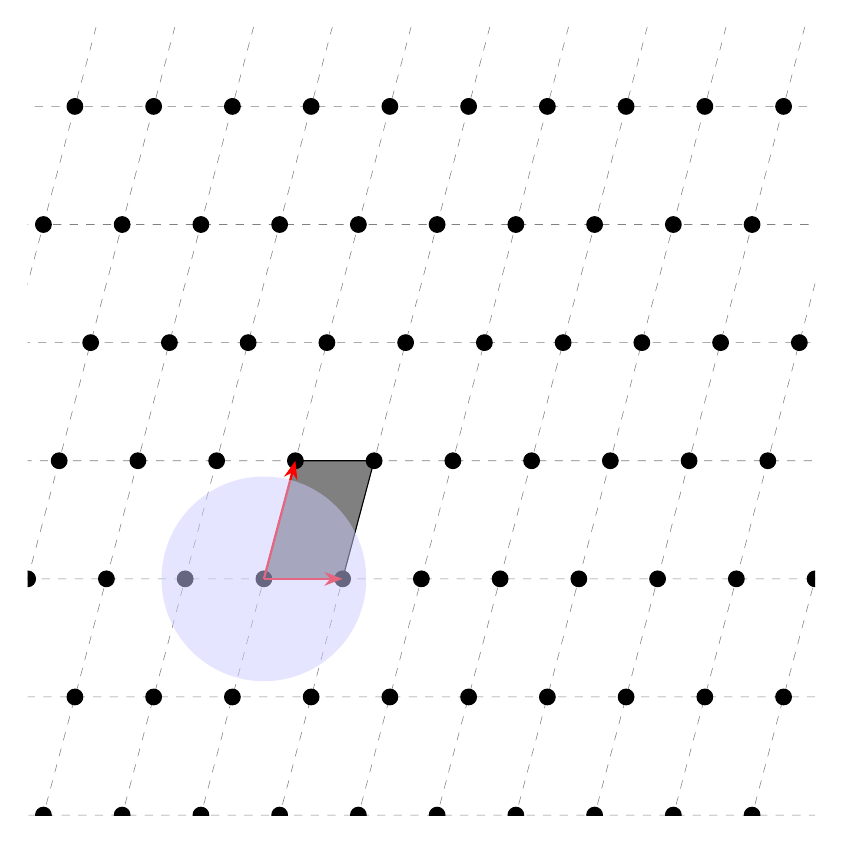
\begin{tikzpicture}
    \begin{scope}
      \clip (0,0) rectangle (10cm,10cm); % Clips the picture...
      \pgftransformcm{1}{0}{0.4}{1.5}{\pgfpoint{3cm}{3cm}} % Adjusted transformation matrix for less skew

      \draw[style=help lines,dashed] (-14,-14) grid[step=1cm] (14,14); % Draws a grid in the new coordinates
      \filldraw[fill=gray, draw=black] (0,0) rectangle (1,1); % Puts the shaded rectangle
      \foreach \x in {-7,-6,...,7}{                           % Two indices running over each
          \foreach \y in {-7,-6,...,7}{                       % node on the grid we have drawn 
              \node[draw,circle,inner sep=2pt,fill] at (\x,\y) {}; % Places a dot at those points
            }
        }
      % Draw the vector from (0,0) to (1,0) in the transformed coordinate system
      \draw[red, -Stealth, thick] (0,0) -- (1,0); % Vector from (0,0) to (1,0)
      \draw[red, -Stealth, thick] (0,0) -- (0,1); % Vector from (0,0) to (0,1)

    \end{scope}
    % Place the circle at the lowest-left vertex (3,3) in the original coordinate system
    \fill[blue!20,semitransparent] (3,3) circle (1.3cm); % Radius is 1.3cm to contain the shorter edge
  \end{tikzpicture}
  \caption{Example of a lattice}
  \label{fig:example}
\end{figure}
Now applying the above process, we get the figure on the left. If we further taking the convex hull of the diagram,
we will get the figure on the right
\begin{figure}[h]
  \centering
  \begin{minipage}{.2\textwidth}
    \begin{tikzpicture}[>=stealth, x=1.1cm, y=1.1cm]
      % Dashed lines (axes)
      \draw[help lines, dashed, ->] (-1,0) -- (3,0);
      \draw[help lines, dashed, ->] (0,-3) -- (0,3);
      \draw[help lines, dashed, ->] (1,-3) -- (1,3);
      \draw[help lines, dashed, ->] (2,-3) -- (2,3);

      % Points (all with fill=blue and radius=0.09cm)
      \filldraw[fill=blue] (2, -0.5) circle[radius=0.09cm];
      \filldraw[fill=blue] (0, 0) circle[radius=0.09cm]; % Removed duplicate
      \filldraw[fill=blue] (1, -0.7) circle[radius=0.09cm];

      \filldraw[fill=blue] (1, -0.3230737092181455) circle[radius=0.09cm];
      \filldraw[fill=blue] (1, 0.12122108098130914) circle[radius=0.09cm];
      \filldraw[fill=blue] (1, 2.28412917072110916) circle[radius=0.09cm];
      \filldraw[fill=blue] (1, 2.3729881287610001) circle[radius=0.09cm];
      \filldraw[fill=blue] (1, 0.4) circle[radius=0.09cm];
      \filldraw[fill=blue] (1, 0.5655158711807637) circle[radius=0.09cm];
      \filldraw[fill=blue] (1, 2.6445016116606668) circle[radius=0.09cm];
      \filldraw[fill=blue] (1, 0.7481703960405396) circle[radius=0.09cm];
      \filldraw[fill=blue] (1, 1.3282219276898275) circle[radius=0.09cm];
      \filldraw[fill=blue] (1, 1.0912647062501184) circle[radius=0.09cm];
      \filldraw[fill=blue] (1, 1.1603772291700336) circle[radius=0.09cm];
      \filldraw[fill=blue] (1, 1.2) circle[radius=0.09cm];
    \end{tikzpicture}~
  \end{minipage} \hspace{3cm} \begin{minipage}{.2\textwidth}
    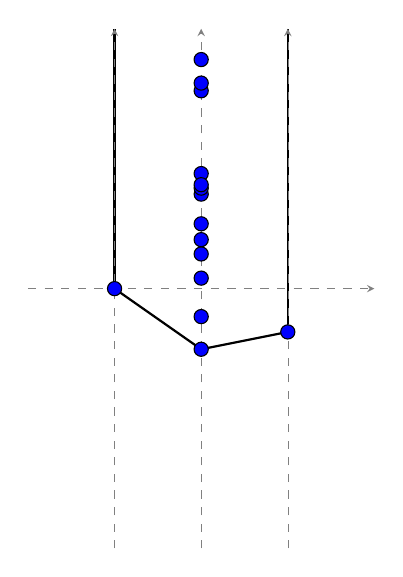
\begin{tikzpicture}[>=stealth, x=1.1cm, y=1.1cm]
      % Dashed lines (axes)
      \draw[help lines, dashed, ->] (-1,0) -- (3,0);
      \draw[thick] (0,0) -- (0,3);
      \draw[thick] (0,0) -- (1, -0.7);
      \draw[thick] (1,-0.7) -- (2,-0.5);
      \draw[thick]  (2,-0.5) -- (2,3);
      \draw[help lines, dashed, ->] (0,-3) -- (0,3);
      \draw[help lines, dashed, ->] (1,-3) -- (1,3);
      \draw[help lines, dashed, ->] (2,-3) -- (2,3);

      % Points (all with fill=blue and radius=0.09cm)
      \filldraw[fill=blue] (2, -0.5) circle[radius=0.09cm];
      \filldraw[fill=blue] (0, 0) circle[radius=0.09cm]; % Removed duplicate
      \filldraw[fill=blue] (1, -0.7) circle[radius=0.09cm];
      \filldraw[fill=blue] (1, -0.3230737092181455) circle[radius=0.09cm];
      \filldraw[fill=blue] (1, 0.12122108098130914) circle[radius=0.09cm];
      \filldraw[fill=blue] (1, 2.28412917072110916) circle[radius=0.09cm];
      \filldraw[fill=blue] (1, 2.3729881287610001) circle[radius=0.09cm];
      \filldraw[fill=blue] (1, 0.4) circle[radius=0.09cm];
      \filldraw[fill=blue] (1, 0.5655158711807637) circle[radius=0.09cm];
      \filldraw[fill=blue] (1, 2.6445016116606668) circle[radius=0.09cm];
      \filldraw[fill=blue] (1, 0.7481703960405396) circle[radius=0.09cm];
      \filldraw[fill=blue] (1, 1.3282219276898275) circle[radius=0.09cm];
      \filldraw[fill=blue] (1, 1.0912647062501184) circle[radius=0.09cm];
      \filldraw[fill=blue] (1, 1.1603772291700336) circle[radius=0.09cm];
      \filldraw[fill=blue] (1, 1.2) circle[radius=0.09cm];
    \end{tikzpicture}~
  \end{minipage}
\end{figure}
Clearly for each dimension, we have the corresponding lowest point, and so the convex hull of
the plot is bounded from below. Grayson calls the plot on the left \textbf{ canonical plot} of the lattice and
the boundary of the convex hull of the canonical plot its \textbf{canonical polygon}. In the expository \cite{}
of Bill Casselman, he instead calls the canonical polygon as \textbf{profile}. We will use the terminology of Casselman.

Now we will try to understand the profile of a lattice associated to a point $z \in \mathfrak{D}$. First we
prove a simple observation
\begin{lemma}
  If $z \in \mathfrak{D}$ then the lattice $L_z = \mathbb{Z}z\oplus \mathbb{Z}$ admits 1 as the shortest vector.
\end{lemma}
\begin{proof}
  We identify $z = x+iy$ with $(x,y) \in \mathbb{R}^2$ and $1$ with $(1,0) \in \mathbb{R}^2$.
  Assume that $1$ is not the shortest vector, then there exists $a,b \in \mathbb{Z}$ such that
  \[ |az+b|^2 < 1 \Leftrightarrow (ax+b)^2+(ay)^2 < 1\Leftrightarrow a^2|z|^2+2abx+b^2< 1\]
  Since $z \in \mathfrak{D}$, we clearly have $|x| \le \frac{1}{2}$ and $|z| \ge 1$,  thus the integers $a,b$ must
  satisfy
  \[ a^2 -|ab|+b^2 < 1\]
  Since the above expression are symmetric, we can assume $|a| \ge |b|$ and completing the square yields
  \[\left(\dfrac{\sqrt{3}b}{2}\right)^2 \ge a^2-ab+b^2 <1 \Rightarrow b^2<4/3 \Rightarrow b \le 1\]
  Substituting $|b|=1$ yields $|a|^2-|a|<0$. There is no non-zero integer $a$ satisfying this condition.
\end{proof}
The area of the lattice $L_z$ is given by $\det\begin{bmatrix}
    y & x \\
    0 & 1
  \end{bmatrix} = y$. Note that we can scale the basis by a factor $a=\sqrt{y}$ so that we get a lattice of volume $1$.
So the lowest points with respect to the axes $x = 0,1,2$ are $(0,0), (1,-\log(a))$, and $(2,0)$.
The interesting part of $\mathfrak{D}$ is where $y\le 1$. This corresponds to the lattices
that have the canonical plots lying entirely on or above the $x$-axis. In particular, the profile of such a lattice
only has the vertices at the origin and $(2,0)$. Grayson and Stuhler call this kind of lattice
\textbf{semi-stable}. If we don't normalize the area of such a lattice, then a semi-stable
lattice has the bottom of the profile as a straight line.

Conversely, the lattices assigned to the points $z \in \uH$ with $\Im(z)>1$ correspond to lattices
that have the canonical plot breaking at the lowest point on the axis $x=1$. In the general case, this reflects the fact that
a non semi-stable lattice has the shortest vector $u$ satisfying $||u||<\sqrt{\vol(L_z)}$. Following Casselman,
we call such a lattice \textbf{unstable}. In some sense, we can see that \textit{the degree of instability} is measured
by the shortest vector compared to its volume. In the above lemma, we only find the semi-stable locus inside the fundamental domain.
To find the semi-stable locus for the whole upper half plane $\uH$, we use the following lemma:
\begin{lemma}
  If $L_z$ is semi-stable, then so is the lattice $L_{g \circ z}$, where $g \in \SLR$.
\end{lemma}
\begin{proof}
  If we denote $L_z=\text{span}_\mathbb{Z}\left\lbrace 1,z\right\rbrace$, then $L_{\gamma\circ z} = cL_z$ for some complex number $c$.
  Indeed, we just need to check for $\gamma$ being an inversion or translation, since these two transformations generate $\SLR(\mathbb{Z})$, but this is easy.
  Now let $c = re^{it}$. Multiplying by $e^{it}$ doesn't change the length, hence doesn't change the semi-stability. Multiplying by a positive number
  $r$ will shift $(1,\log|u|)$ to $(1,\log|u|+\log r)$ and $(2,\log(\vol(A)))$ to $(2,\log(\vol(A))+2\log r)$.

  \todo{I think in 2-dimensional case, c is 1}

  The line segment $d$ connecting the origin with the final point intersects the line $x=1$ at $(1,\log(\vol(A))+\log r)$. By the semi-stability of the original lattice,
  the point $(1,\log|u|+\log r)$ is above the line segment $d$.
\end{proof}
From this lemma, we can see that the semi-stable locus is the complement of the Farey balls in the upper half plane, as illustrated in the
following figure, where the blue part is the semi-stable locus and the gray part is the unstable one.
\begin{figure}[h]
  \centering
  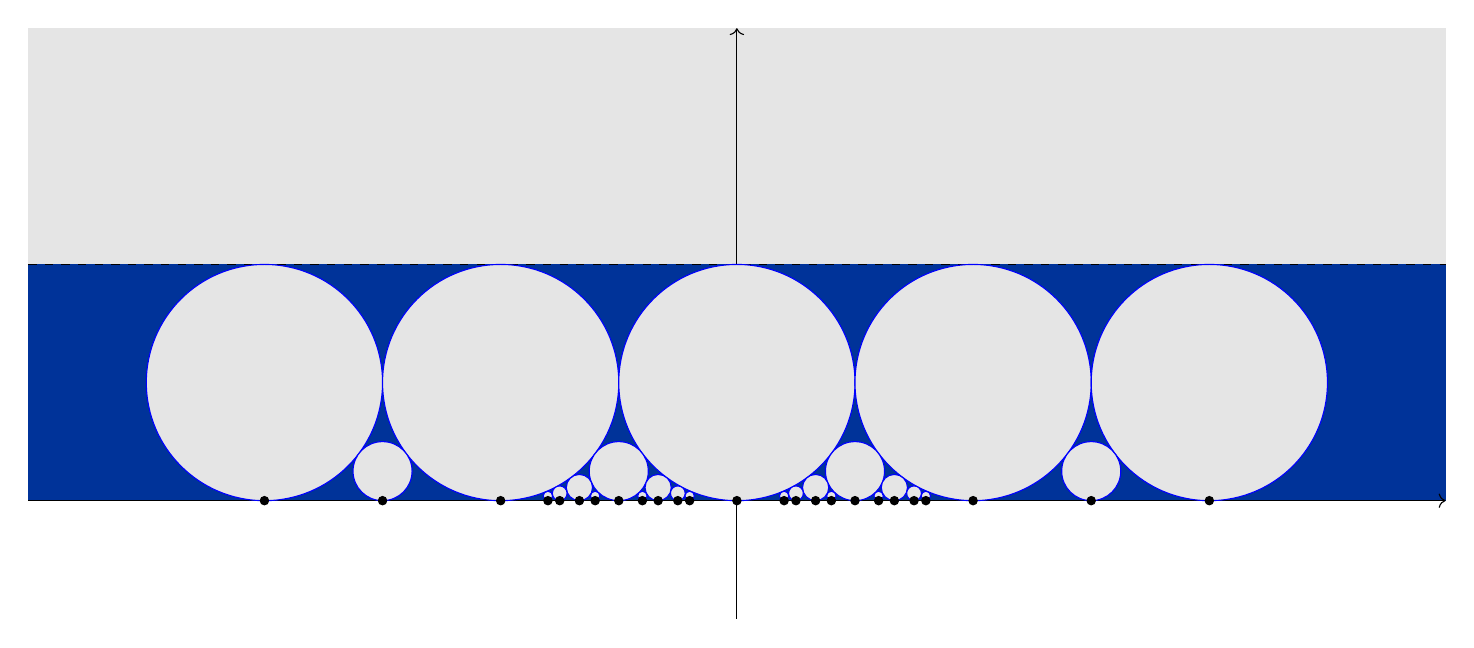
\begin{tikzpicture}[scale =3]
    % Define colors
    \definecolor{sapphire}{rgb}{0, 0.2, 0.6} % A deep blue for the region y < 1

    % Fill the entire visible area with sapphire (y < 1 region)
    \fill[sapphire] (-3, 0) rectangle (3, 1);

    % Fill the region y >= 1 with gray
    \fill[gray!20] (-3, 1) rectangle (3, 2);

    % Draw the x-axis and y-axis (without labels)
    \draw[->] (-3, 0) -- (3, 0);
    \draw[->] (0, -0.5) -- (0, 2);

    % Draw the line y = 1 (without label)
    \draw[dashed] (-3, 1) -- (3, 1);

    % Define a macro to draw a circle at (p/q, 0) with radius 1/(2q^2)
    \def\drawCircle#1#2{ % #1 = p, #2 = q
      \pgfmathsetmacro{\pq}{#1/(#2)} % Compute p/q
      \pgfmathsetmacro{\radius}{1/(2*(#2)^2)} % Compute radius = 1/(2q^2)
      \filldraw[fill=gray!20, draw=blue] (\pq, \radius) circle[radius=\radius cm]; % Fill with gray, outline in blue
      \filldraw[black] (\pq, 0) circle[radius=0.5pt]; % Mark the point (p/q, 0) with a smaller dot
    }

    % Draw circles for specific coprime pairs (p, q)
    % q = 1
    \drawCircle{-2}{1}
    \drawCircle{-1}{1}
    \drawCircle{0}{1}
    \drawCircle{1}{1}
    \drawCircle{2}{1}

    % q = 2
    \drawCircle{-3}{2}
    \drawCircle{-1}{2}
    \drawCircle{1}{2}
    \drawCircle{3}{2}

    % q = 3
    \drawCircle{-2}{3}
    \drawCircle{-1}{3}
    \drawCircle{1}{3}
    \drawCircle{2}{3}

    % q = 4
    \drawCircle{-3}{4}
    \drawCircle{-1}{4}
    \drawCircle{1}{4}
    \drawCircle{3}{4}

    % q = 5
    \drawCircle{-4}{5}
    \drawCircle{-3}{5}
    \drawCircle{-2}{5}
    \drawCircle{-1}{5}
    \drawCircle{1}{5}
    \drawCircle{2}{5}
    \drawCircle{3}{5}
    \drawCircle{4}{5}
  \end{tikzpicture}
  \caption{Semistable locus in upper half plane}
  \label{P-partition}
\end{figure}
\section{$\rho$-semi-stability of lattices}
The semi-stability can be defined in a more Lie-theoretic way. First we recall the Iwasawa decomposition
for $\SLR$.
\begin{prop}
  We have
  \[\SLR \cong K \times A \times N\]
  where
  \begin{itemize}
    \item $K=\SO2$: the special orthogonal group.
    \item $A = \left\lbrace \begin{bmatrix}
              a & 0      \\
              0 & a^{-1}
            \end{bmatrix}: a >0 \right\rbrace$.
    \item  $N = \left\lbrace \begin{bmatrix}
              1 & b \\
              0 & 1
            \end{bmatrix}\right\rbrace$.
  \end{itemize}
\end{prop}
Combinining with Proposition \ref{h-as-matrices}, we have the following identification
\[\uH \cong A \times N\]
via the map
\[x+iy \mapsto \begin{bmatrix}
    1/\sqrt{y} & 0        \\
    0          & \sqrt{y}
  \end{bmatrix}\begin{bmatrix}
    1 & -x \\
    0 & 1
  \end{bmatrix} = a\left(y\right)n(x)\]
Let's denote $\sl2$ the Lie algebra of the Lie group $\SLR$ - the vector space of traceless matrices of size $2 \times 2$. We denote
$\mathfrak{h} = \mathbb{R}H$ where $H =\begin{bmatrix}
    1 & 0  \\
    0 & -1
  \end{bmatrix}$ its standard Cartan subalgebra. We then have the map
\begin{align*}
  H_B \colon \uH \to \mathfrak{h}, \quad
  z = x+iy \mapsto \log(a(y))H = \frac{-1}{2}\log(\Im(z))
\end{align*}
Let $\alpha\colon \mathfrak{h} \to \mathbb{R}$ be the unique linear function such that
$\alpha(H)=2$. If we let $\rho = \dfrac{1}{2}\alpha$, then we define
\[\deg_{\text{inst}}(z):= \min_{\gamma \in  \Gamma/\Gamma \cap B} \left\langle \rho,H_B(z\gamma) \right\rangle\]
where $B$ is the group of upper triangular matrices with invertible entries along the diagonal.
\begin{definition}
  The lattice $L_z$ corresponds to the point $z \in \uH$ is called \textbf{$\rho$-semistable} or just \textbf{semi-stable}
  if $\deg_{inst}(z) \ge 0$.
\end{definition}
We shall use this definition to find the semi-stable locus in the upper half plane $\uH$.
\begin{prop}
  The locus of $\rho$-semistable points in the upper half plane $\uH$ is the
  complement of the Farey balls.
\end{prop}
\begin{proof}
  We first make simple observation: If $\deg_{\text{inst}}(z)$ is achieved at some
  $\gamma_0 \in \Gamma$ and $z$ is $\rho$-semistable, then
  \[\left\langle \rho, H_B(z\gamma)\right\rangle \ge 0 \mbox{ for all } \gamma \in \Gamma\]
  From this observation, the $\rho$-semistable locus must be the set
  \[ \left\lbrace z \in \uH: \left\langle \rho, H_B(z\gamma)\right\rangle \ge 0 \mbox{ for all } \gamma \in \Gamma \right\rbrace\]
  We identify $z=x+iy$ with the product $a(y)n(x)$ as above. Under the identification \ref{upper-group}, we must have
  \[\left\langle \rho, H_B(z\gamma) = -\log(a(\gamma^{-1} \circ z)) \right\rangle\]
  Assume that $\gamma^{-1} =
    \begin{bmatrix}
      a & b \\
      c & d
    \end{bmatrix}$, then $\gamma^{-1} \circ z$ satisfies
  \[\Im(\gamma^{-1}\circ z) = \dfrac{\Im(z)}{(cx+d)^2+(cy)^2}\]
  Thus, $z$ is semistable if and only if it satifies the inequalities
  \[y \le(cx+d)^2+(cy)^2  \Leftrightarrow \left(x+\dfrac{c}{d}\right)^2+\left(y-\dfrac{1}{2c^2}\right)^2 \ge \left(\dfrac{1}{2c^2}\right)^2 \]
  for any $c,d$ coprime. Since the above equation is exactly the equation for Farey balls, we are done.
\end{proof}
In particular, we just proved that the $\rho$-semistablility and the semistablility in Grayson's sense
are equivalent.
\subsection{Unstable lattices}
Consider an unstable lattice $L$ with a shortest vectur $u$, then the bottom
of the profile of $L$ has a break at the point $(1,\log(||u||))$. Clearly $u$ is a primitive vector, so $L_1 = \mathbb{Z}u$
is a sublattice of $L$. This determines a \textbf{lattice flag}
\[\mathcal{F}: 0 \subset L_1 \subset L_2 = L\]
And this is called the \textbf{canonical flag} associated to $L$. By tensoring with $\mathbb{R}$ we get
a flag of rational subspaces
\[0 \subset V_1 = L_1 \otimes \mathbb{R} \subset V_2 = L_2 \otimes \mathbb{R}\]
Conversely, for any rational flag $\mathcal{F}$ in $\mathbb{R}^2$, we can denote $\mathcal{H}_\mathcal{F}$ the set of all
unstable lattices that gives rise to the flag $\mathcal{F}$. What can we say about the set
$\mathcal{H}_\mathcal{F}$? It turns out that the can be parametrized by the Farey balls in the complex plane.
\begin{prop}
  Given a flag of rational vector spaces
  \[\mathcal{F}: 0 \subset V_1 \subset V_2 =\mathbb{R}^2\]
  Assume that $V_1 = \text{span}(pf_1+qf_2)$ for some $\mathbb{R}$- linearly independent set $\{f_1,f_2\}$ . Then
  the set $\mathcal{H}_\mathcal{F}$ corresponds to the Farey balls that is tangent to the $x-axis$ at the fraction $p/q$.
  Morever, each Farey circle corresponds to the set of lattices with the same profiles.
\end{prop}
\begin{figure}[h]
  \centering
  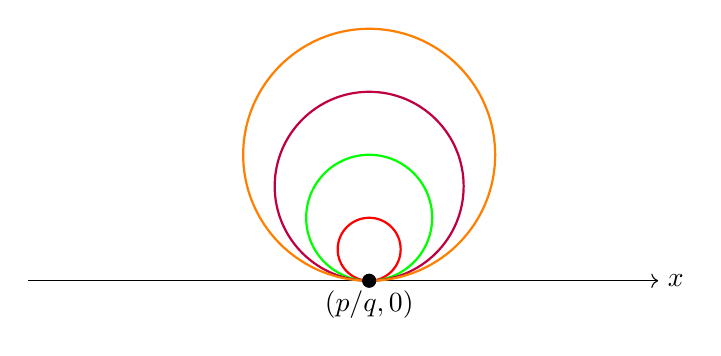
\begin{tikzpicture}[scale =10]
    % Draw the x-axis
    \draw[->] (-0.1,0) -- (0.7,0) node[right] {$x$};

    % Draw the enlarged Ford circle for 1/3
    % Original radius: 1/(2*3^2) = 0.0556, scaled by 2: 0.1112
    % Center: (1/3, 0.1112) ≈ (0.333, 0.1112)
    \node[below] at (0.333,0) {};

    % Draw four additional enlarged circles tangent at (1/3, 0)
    % Circle 2: original radius 0.02, scaled to 0.04, center (0.333, 0.04)
    \draw[red, thick] (0.333,0.04) circle (0.04);
    % Circle 3: original radius 0.04, scaled to 0.08, center (0.333, 0.08)
    \draw[green, thick] (0.333,0.08) circle (0.08);
    % Circle 4: original radius 0.06, scaled to 0.12, center (0.333, 0.12)
    \draw[purple, thick] (0.333,0.12) circle (0.12);
    % Circle 5: original radius 0.08, scaled to 0.16, center (0.333, 0.16)
    \draw[orange, thick] (0.333,0.16) circle (0.16);

    % Mark the tangency point
    \fill (0.333,0) circle (0.009);
    \node[below] at (0.333,0) {$(p/q,0)$};
  \end{tikzpicture}
  \caption{The Farey Circles correspond to the same rational flag}
  \label{P-coordinate}
\end{figure}
\begin{proof}
  Consider the lattice $L=L_z \in \mathcal{H}_\mathcal{F}$ for $z = x+iy$. This lattice $L$ has a basis
  \[\begin{cases}
      f_1 = \dfrac{e_1}{\sqrt{y}} \\
      f_2 = \dfrac{-xe_1}{\sqrt{y}}+e_2\sqrt{y}
    \end{cases}\]
  Assume that $u=pf_1+qf_2$ is the shortest vector of $L$. Since $u$ is primitive, we must have $\gcd(p,q)=1$. Since the lattice
  $L$ is unstable, it follows that $\mu(L_1) \le \mu(L/L_1)$ for $L_1 = \mathbb{Z}u$. In particular, we have
  \[\dfrac{|-qz+p|}{\sqrt{y}} \le 1 \Leftrightarrow (-qx+p)^2 +(qy)^2 \le y \]
  If $q \ne 0$, this is the equation for the Farey balls that tangent to the horizonal axis at $(p/q,0)$. If $p=0$ then $q=1$, the equation
  $\dfrac{|-qz+p|}{\sqrt{y}} \le 1$ degenerates to $y \ge 1$. Hence we are done.
\end{proof}
\begin{remark}
  Note that for every flag in $\mathbb{R}^2$ corresponds to a parabolic subgroup. For example, the subgroup 
  \[B = \begin{bmatrix}
    1 & n \\
    0 & 1
  \end{bmatrix}\]
  stabilizes the flag $0 \subset \mathbb{R}e_1 \subset \mathbb{R}^2$ for some choice of basis $\{e_1,e_2\}$ of $\mathbb{R}^2$. Any parabolic subgroup of $\SLR$ is conjugate with $B$. So there is a correspondence between 
  rational parabolic subgroups of $\SLR$, that is, the parabolic subgroup that stabilizes a rational flag $\mathcal{F}$ - and the collections $\mathcal{H}_\mathcal{F}$ of lattices 
  gives rise to the flag $\mathcal{F}$. 
\end{remark}



\chapter{ROOTS AND WEIGHTS FOR $\SLn$/$\GLn$}
 % Sets article title
In this chapter, we review some basic theory of roots and weight. We will first recall the
general theory and compute explicitly the examples for $\SLn$/$\GLn$.
\section{Structure theory}
\subsection{The Cartan subalgebra}
First we need the notion of Cartan subalgebra
\begin{definition}
    For any Lie algebra $\mathfrak{g}$, a subalgebra $\mathfrak{h}$ of $\fg$ is said to be a \textit{Cartan algebra} if it is
    \begin{itemize}
        \item $\fh$ is a nilpotent subalgebra.
        \item It is self normalizing. In particular, we have $\fh = \left\lbrace x \in \fg : [x,\fg] \subset \fg\right\rbrace$.
    \end{itemize}
\end{definition}
When $\fg$ is a semisimple Lie algebra, we have the following theorem
\begin{theorem}
    Let $\fg$ be a semisimple Lie algebra over an algebraically closed field $k$ of characteristic $0$ with a subalgebra $\fh$.
    Then $\fh$ is a Cartan subalgebra of $\fg$ if and only if it is a maximal toral subalgebra, i.e. is maximal among all subalgebras
    containing only semisimple elements.
\end{theorem}\todo{add citation.}
\subsection{Root space decomposition}
With respect to some choice of Cartan subalgebra, we have a root space decomposition. In particular, there is a finite set
$\Phi \subset \fh^{*}$ of linear forms on $\fh$, whose elements are called \textbf{roots}, such that
\[\fg = \fh \oplus \left(\bigoplus_{\alpha \in \Phi} \mathfrak{g}_\alpha\right),\]
where $\fg_\alpha = \left\lbrace x \in \fg: [h,x] = \alpha(h)x, \forall h \in \fh\right\rbrace$ for any $\alpha \in \Phi$.
\subsection{A specific example: root space decomposition for $\mathfrak{sl}_n(\mathbb{R})$}
For the semisimple Lie algebra $\slnr$, a typical choice of the Cartan subalgebra is the set
\[\fh = \left\lbrace H= \begin{bmatrix}
        a_1    & 0      & \ldots & 0      \\
        0      & a_2    & \ldots & 0      \\
        \vdots & \vdots & \ddots & \vdots \\
        0      & 0      & \cdots & a_n
    \end{bmatrix}, a_1 + a_2+ \ldots + a_n = 0\right\rbrace\]
With respect to this Cartan subalgebra, we can define the linear function
\[L_i \colon \fh \to \mathbb{R}, \quad H \mapsto L_i(H)= a_i\]
Then the roots are given by $\alpha_{ij} :=L_i - L_j$ for distinct $i,j$. We have the root space decomposition for $\slnr$ as follows
\[\fg = \fh \oplus \left(\bigoplus\fg_{\alpha_{ij}}\right).\]
For the sake of brevity, we will denote $\alpha_{i,i+1}$ by $\alpha_i$ - these are called \textbf{simple roots}.
\subsection{Roots at group level}
Since the main object in this thesis is the Lie groups, we want to understand how the roots
behave at group level. The analog for the Cartan subalgebra is the maximal torus
\[T = \left\lbrace t= \begin{bmatrix}
        a_1    & 0      & \ldots & 0      \\
        0      & a_2    & \ldots & 0      \\
        \vdots & \vdots & \ddots & \vdots \\
        0      & 0      & \cdots & a_n
    \end{bmatrix} :  a_i \ne 0\right\rbrace,\]
Then $T$ acts on $\fg$ by conjugation. Explicitly, we can check that
\[\Ad(t)(E_{ij}) = t_it_j^{-1}E_{ij}\]
Therefore, at the group level, the character $\alpha_{ij}(\text{diag}(t_1,\ldots,t_n))=t_it_j^{-1}$
is a root whenever $i \ne j$. The set
\[\Delta = \left\lbrace \alpha_i\mid i =\overline{1,n}\right\rbrace\]
where
\[\alpha_i \colon T \mapsto \mathbb{R}, t \mapsto \dfrac{t_i}{t_{i+1}}\]
is the set of \textbf{simple roots}.
We can decompose the set of root into to disjoint subsets, namely
\[\Phi = \left\lbrace \alpha_{ij}, i \ne j\right\rbrace = \Phi_+ \coprod \Phi_{-}\]
where the set $\Phi_+$ comprises $\alpha_{ij}$ for $i<j$ and the remaining roots are in $\Phi_{-}$. The former consists of
\textbf{positive roots} while the latter contains \textbf{negative roots}. We have the following lemma
\begin{lemma}\label{linear-comb-of-roots}
    Each $\alpha \in \Phi$ can be written uniquely as a linear combination
    \[\alpha = m_1\alpha_1+\ldots+m_{d}\alpha_{d}\]
    with all $m_i \in \mathbb{Z}_{\ge 0}$ or $m_i \in \mathbb{Z}_{\le 0}$. If $\alpha \in \Phi_+$ then all $m_i \ge 0$, otherwise $m_i \le 0$ for all $i$.
\end{lemma}
\subsection{Weights}
\todo{define in terms of Lie algebra}
Another class of linear forms that we are interested in are the \textbf{fundamental weights}. For each fundamental
weights $\lambda_i$, we define
\[\lambda_i \colon T \to \mathbb{R}, \quad\lambda_i(t) = a_1\ldots a_i\]
We have the following
\begin{lemma}\label{linear-comb-of-weights}
    We can write
    \[\lambda_i := r_1\alpha_1 + r_2\alpha_2+\ldots + r_d\alpha_d\]
    where $r_i$'s are rational number such that $r_i \ge 0$.
\end{lemma}
This coefficients $r_i$'s is determined by inverting the Cartan matrix of $\slnr$. Hence we postpone a proof
of this until reviewing the notion of Cartan matrices.
\begin{example}
    When $n=3$, we have the following relations 
    \[\lambda_1 = \dfrac{2}{3}\alpha_1+\dfrac{1}{3}\alpha_2, \quad \lambda_2 = \dfrac{1}{3}\alpha_1+\dfrac{2}{3}\alpha_2\]
\end{example}
\begin{figure}[h]
    \centering
    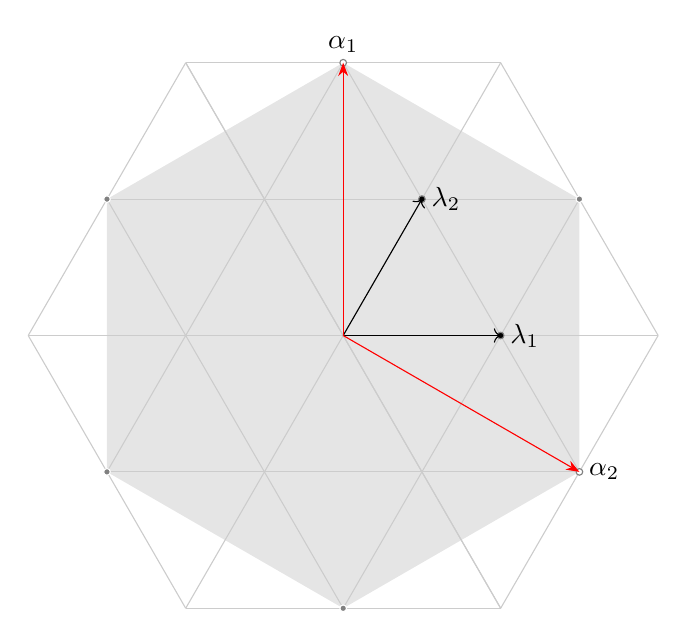
\begin{tikzpicture}
        \begin{rootSystem}[weight length=2cm]{A}
            \roots
            \simpleroots
            \node [above] at \Root {1}{0} {\(\alpha_1\)};
            \node [right] at \Root {0}{1} {\(\alpha_2\)};
            \fundamentalweights
            \node [right] at \weight {1}{0} {\(\lambda_1\)};
            \node [right] at \weight {0}{1} {\(\lambda_2\)};
            \draw[->] (0,0)--\weight{1}{0};
            \draw[->] (0,0)--\weight{0}{1};
            \draw [red, arrows = {-Stealth}] (0,0)--\Root {1}{0};
            \draw [red, arrows = {-Stealth}] (0,0)--\Root {0}{1};
        \end{rootSystem}
    \end{tikzpicture}
    \caption{Roots and weights for the Lie group $\text{SL}_3(\mathbb{R})$}
\end{figure}


\begin{definition}
    A weight $\lambda$ is called \textbf{dominant} if it satisfies $\left\langle \lambda,\alpha^{\vee} \right\rangle \in \mathbb{Z}_{\ge 0}$ for all $\alpha$
\end{definition}
Clearly by lemma \ref{linear-comb-of-roots}, the weight $\lambda$ is dominant if and only if $\left\langle\lambda,\alpha_i^\vee\right\rangle$ for all
fundamental root $\alpha_i$. It is also clearly that the set of fundamental weight is given by addition of the fundamental weights, namely
\[\Lambda^+ := \left\lbrace c_1\lambda_1+\ldots+c_d\lambda_d \mid c_i \in \mathbb{Z}_{\ge 0}\right\rbrace\]
The set of dominant weights is denoted $\Lambda^+$. A weight $\lambda = \sum n_i \lambda_i$ is called strongly dominant if $n_i > 0$ for all $i$. One important example is the minimal strongly dominant weight given by
\[
    \rho = \sum \lambda_i
\]
This is called \textbf{Weyl vector} and is characterized in several ways:

\begin{enumerate}
    \item $\left\langle\rho,\alpha_i^\vee\right\rangle = 1$ for all $i$.
    \item
          \[
              \rho = \frac{1}{2} \sum_{\alpha \in \Phi^+} \alpha
          \]
\end{enumerate}

To prove the last equation we use the action of the Weyl group $W$. Let $\mu = \frac{1}{2} \sum \alpha$. Apply the simple reflection $s_i$ given by
\[
    s_i(x) = x - \left\langle x, \alpha_i^\vee\right\rangle \alpha_i
\]
We know that $s_i$ sends $\alpha_i$ to $-\alpha_i$ and permutes the other positive roots. So:
\[
    s_i(\mu) = \mu -  \left\langle x, \alpha_i^\vee\right\rangle  \alpha_i
\]
Therefore, $(\mu, \alpha_i) = \mu(h_i) = 1$ for all $i$. So, $\mu = \rho$.

Unlike lemma \ref{linear-comb-of-weights}, if we try to express the fundamental weights in terms of the fundamental roots, we don't always
get positive coefficients. However, it is true that all the coefficients must be integer. In particular, we have
\[\alpha_j = \sum_{n_j}\lambda_j, \quad n_j \in \mathbb{Z}.\]
To put it another way, the root lattice $\mathbb{Z}\Delta$ is contained inside the weight lattice.
\subsection{Weyl group}
We only define the Weyl group explicitly for the group $\SLn$ or $\GLn$. It is a fact that the Weyl groups for
these two Lie groups are the same and equal to $W = S_n$ - the permutation group of $n$ letters.  We recall some basis
observation about this group
\begin{enumerate}
    \item Every $\sigma \in W$ can be written (non-uniquely) as a product of $w_{i_1} \cdots w_{i_k}$ for some integer $k$. Such a sequence is said to have length $k.$ If $k$ is the minimum, over all such writings, it is called the length of $\sigma$ and written $\ell(\sigma)$. Any expression of length $\ell(\sigma)$ for $\sigma$ is called a reduced expression.

    \item The group $S_n$ is generated by $S$ subject to the following two types of relations:
          \begin{itemize}
              \item (Reflection) $w_i^2=1$ for $i \in I$.
              \item (Braid relations) $w_i \, w_{i+1} \, w_i = w_{i+1}w_i w_{i+1}$ for $i = 1, \ldots, n-2$ and $w_i w_j = w_j w_i$ for $|j -i |\geq 2$.
          \end{itemize}
\end{enumerate}
Note that $W$ acts on $\Hom(H, \mathbb{R}^*)$ in the natural way: $w . \varphi(h) = \varphi(w^{-1} h)$. More explicitly,  $\sigma$ sens $\alpha:= \alpha_{ij}$ to $\alpha_{\sigma(i), \sigma(j)}$. Hence we find that
\[w_i \alpha_j = \begin{cases} - \alpha_i          & \mbox{if } i=j           \\
              \alpha_j            & \mbox{ if } |j - i | > 1 \\
              \alpha_i + \alpha_j & \mbox{ if } |j-i|=1\end{cases} \]
We of course also have an action of $W$ on the weights.  For example, one can verify that
\[ \begin{array}{lcr} s_i(\lambda_i) = \lambda_i - \alpha_i & \text{ and } & s_j(\lambda_i) = \lambda_i \mbox{ for } i \neq j \end{array}.\]
Recall the definition of Weyl vector $\rho$, we have the following generalized action of Weyl group of $\rho$:
\[ w \rho = \rho - \sum_{\alpha \in \Delta_{w^{-1}}} \alpha,\]
where \textcolor{red}{check this explicitly}
\[\Delta_{\sigma}:= \{ \alpha \in \Phi_+ \mid \sigma(\alpha) \in \Phi_- \}\]
\subsection{Cartan matrix}
We fix a set of simple roots $\Delta = \left\lbrace \alpha_1,\ldots,\alpha_d \right\rbrace$ is defined to be the matrix
\[A = \begin{bmatrix} \left\langle \alpha_i,\alpha_j^\vee  \right\rangle
    \end{bmatrix}\]
If we let $a_{ij}=  \left\langle \alpha_i,\alpha_j^\vee\right\rangle$ then the Cartan matrix has the following simple properties:
\begin{lemma}
    \hfill
    \begin{itemize}
        \item For any $i$, we have $a_{ii}=2$.
        \item For any $i \ne j$, $a_{ij}$ is a non-positive integer, i.e. $a_{ij} \in \mathbb{Z}_{\le 0}$.
    \end{itemize}
\end{lemma}
We give an explicit example for $\slnr$, which has the root system $A_n$. The corresponding Cartan matrix is
\[A_n = \begin{bmatrix}
        2      & -1     & 0      & 0      & \ldots & 0      \\
        -1     & 2      & -1     & 0      & \ldots & 0      \\
        \vdots & \vdots & \vdots & \vdots & \ddots & \vdots \\
        0      & 0      & \ldots & -1     & 2      & -1     \\
        0      & 0      & \ldots & 0      & -1     & 2      \\
    \end{bmatrix}\]
The Cartan matrix provides a linear combination presentation of the fundamental roots $\alpha_j$'s in terms of fundamental weights $\lambda_i$,
as stated in the following lemma
\begin{lemma}\label{weight-root-comb}
    Fix a number $n$ and consider the set of fundamental roots $\alpha_j$ as well as the set of weights $\lambda_i$ of $\SLn$, we have the following relations
    \[\alpha_i = \begin{cases}
            2\lambda_1-\lambda_2,                    & \mbox{ if } i = 1 \\
            -\lambda_{i-1}+2\lambda_i-\lambda_{i+1}, & \mbox{ if } 1<i<n \\
            -\lambda_{n-1}+2\lambda_n,               & \mbox{ if } i =n
        \end{cases}.\]
\end{lemma}
\begin{proof}
    Note that we have
    \[\left\langle \alpha_i,\alpha_j^{\vee}\right\rangle = \begin{cases}
            2, \mbox{ if } i =j     \\
            -1, \mbox{ if } |i-j|=1 \\
            0, \mbox{ otherwise }
        \end{cases}. \]
    So if we let $\alpha_j = \sum_{i=1}^n a_{ij}\lambda_i$ and compute $\left\langle \alpha_i,\alpha_j^{\vee}\right\rangle$, the result follows immediately.
\end{proof}
We will also need the inverse of the Cartan matrices of type $A_n$. The following formulae for the
inverse matrices of $\slnr$ can be found in \cite{}
\begin{theorem}
    The inverse of the Cartan matrices
    \[A_n = \begin{bmatrix}
            2      & -1     & 0      & 0      & \ldots & 0      \\
            -1     & 2      & -1     & 0      & \ldots & 0      \\
            \vdots & \vdots & \vdots & \vdots & \ddots & \vdots \\
            0      & 0      & \ldots & -1     & 2      & -1     \\
            0      & 0      & \ldots & 0      & -1     & 2      \\
        \end{bmatrix},\]
    is the matrix $(A_n)^{-1}$ with the entries given by the following formula
    \[(A_n)^{-1}_{ij} = \min\{i,j\}-\dfrac{ij}{n+1}\]
    As a consequence, we can see that the entries for the inverse matrix $(A_n)^{-1}$ is positive. Indeed, assume that
    $i \ge j$, we have
    \[(A_n)^{-1}_{ij} = \dfrac{j(n+1-i)}{n+1}>0\]
    In particular, we just proved lemma $\ref{linear-comb-of-weights}$.
\end{theorem}
\section{Parabolic subgroups}
We shall provide two equivalent viewpoints on parabolic subgroups. They will play different roles in defining
different notions of semi-stability in the next chapter.
\subsection{Parabolic subgroups I: An explicit description }
For our purposes, it is enough to define the standard parabolic subgroups.  There exists a bijection between each parabolic subgroup of $\SLn$
and each partition of $n$. We can therefore define the parabolic subgroup explicitly as follows:
\begin{definition}
    The standard parabolic subgroup associated to the partition $n = n_1 + n_2 + \cdots + n_r$ is denoted $P_{n_1,\ldots,n_r}$ and is defined to be the group of all matrices of the form
    \[
        \begin{bmatrix}
            \mathfrak{m}_1 & 0              & \ldots & 0              \\
            0              & \mathfrak{m}_2 & \ldots & 0              \\
            \vdots         & \vdots         & \ddots & \vdots         \\
            0              & 0              & \ldots & \mathfrak{m}_k
        \end{bmatrix} ,
    \]
    where $m_{n_i} \in \mathrm{GL}(n_i, \mathbb{R})$ for $1 \leq i \leq r$. The integer $r$ is called the rank of the parabolic subgroup $P_{n_1,\ldots,n_r}$.
\end{definition}

\begin{definition}
    The maximal standard parabolic subgroups in $\text{GL}_n(k)$ corresponds to the
    stabilizer of the flag of type $\rho_i =(i,n-i)$, where $i = 1,\ldots,n-1$ of $n$. We will
    further denote $Q_i = P_{\rho_i}$ and $\textbf{MaxParSt}$ the collection of such maximal parabolic subgroups.
\end{definition}

\begin{example}
    Below we list all the standard parabolic subgroup in $\text{GL}_3(\mathbb{R})$ and $\text{GL}_4(\mathbb{R})$.
    \begin{itemize}
        \item For $\text{GL}_3(\mathbb{R})$, there are three standard parabolic subgroups corresponding to
              three partitions of $3$, namely
              \[ 3 = 1+ 1+ 1, \quad 3 =1+2 , \quad 3 = 2+1\]
              For a partition $(r_1,\ldots,r_{s+1})$, we denote $P_{(r_1,\ldots,r_{s+1})}$ the corresponding parabolic subgroups. Thus, we have
              \begin{align*}
                   & P_{1,1,1} = \left\lbrace \begin{bmatrix}
                                                  \ast & \ast & \ast \\
                                                  0    & \ast & \ast \\
                                                  0    & 0    & \ast
                                              \end{bmatrix}\right\rbrace, \quad P_{1,2} =\left\lbrace \begin{bmatrix}
                                                                                                          \ast & \ast & \ast \\
                                                                                                          0    & \ast & \ast \\
                                                                                                          0    & \ast & \ast
                                                                                                      \end{bmatrix}\right\rbrace \\
                   & P_{2,1} = \left\lbrace \begin{bmatrix}
                                                \ast & \ast & \ast \\
                                                \ast & \ast & \ast \\
                                                0    & 0    & \ast
                                            \end{bmatrix}\right\rbrace
              \end{align*}
              Clearly $\textbf{MaxParSt} = \left\lbrace P_{2,1}, P_{1,2}\right\rbrace$.
        \item For  $\text{GL}_4(\mathbb{R})$, there are seven standard parabolic subgroups for seven partitions
              \[ 4 = 1+ 1+1+1, \quad 4 =1+1+2, \quad 4 = 1+2+1\]
              \[4 =2+1+1, \quad 4 = 1+3, \quad 4 = 2+1, \quad 4 = 3+1\]
              Explicitly, we have the following subgroups
              \begin{align*}
                   & P_{1,1,1,1} = \left\lbrace \begin{bmatrix}
                                                    \ast & \ast & \ast & \ast \\
                                                    0    & \ast & \ast & \ast \\
                                                    0    & 0    & \ast & \ast \\
                                                    0    & 0    & 0    & \ast \\
                                                \end{bmatrix} \right\rbrace, \quad & P_{1,1,2} = \left\lbrace \begin{bmatrix}
                                                                                                                  \ast & \ast & \ast & \ast \\
                                                                                                                  0    & \ast & \ast & \ast \\
                                                                                                                  0    & 0    & \ast & \ast \\
                                                                                                                  0    & 0    & \ast & \ast \\
                                                                                                              \end{bmatrix} \right\rbrace \\
                   & P_{1,2,1} = \left\lbrace \begin{bmatrix}
                                                  \ast & \ast & \ast & \ast \\
                                                  0    & \ast & \ast & \ast \\
                                                  0    & \ast & \ast & \ast \\
                                                  0    & 0    & 0    & \ast \\
                                              \end{bmatrix} \right\rbrace, \quad   & P_{2,1,1} = \left\lbrace \begin{bmatrix}
                                                                                                                  \ast & \ast & \ast & \ast \\
                                                                                                                  \ast & \ast & \ast & \ast \\
                                                                                                                  0    & 0    & \ast & \ast \\
                                                                                                                  0    & 0    & 0    & \ast \\
                                                                                                              \end{bmatrix} \right\rbrace \\
                   & P_{1,2,1} = \left\lbrace \begin{bmatrix}
                                                  \ast & \ast & \ast & \ast \\
                                                  0    & \ast & \ast & \ast \\
                                                  0    & \ast & \ast & \ast \\
                                                  0    & 0    & 0    & \ast \\
                                              \end{bmatrix} \right\rbrace, \quad   & P_{2,1,1} = \left\lbrace \begin{bmatrix}
                                                                                                                  \ast & \ast & \ast & \ast \\
                                                                                                                  \ast & \ast & \ast & \ast \\
                                                                                                                  0    & 0    & \ast & \ast \\
                                                                                                                  0    & 0    & 0    & \ast \\
                                                                                                              \end{bmatrix} \right\rbrace \\
                   & P_{1,3} = \left\lbrace \begin{bmatrix}
                                                \ast & \ast & \ast & \ast \\
                                                0    & \ast & \ast & \ast \\
                                                0    & \ast & \ast & \ast \\
                                                0    & \ast & \ast & \ast \\
                                            \end{bmatrix} \right\rbrace, \quad     & P_{3,1} = \left\lbrace \begin{bmatrix}
                                                                                                                \ast & \ast & \ast & \ast \\
                                                                                                                \ast & \ast & \ast & \ast \\
                                                                                                                \ast & \ast & \ast & \ast \\
                                                                                                                0    & 0    & 0    & \ast \\
                                                                                                            \end{bmatrix} \right\rbrace   \\
                   & P_{2,2} = \left\lbrace \begin{bmatrix}
                                                \ast & \ast & \ast & \ast \\
                                                \ast & \ast & \ast & \ast \\
                                                0    & 0    & \ast & \ast \\
                                                0    & 0    & \ast & \ast \\
                                            \end{bmatrix} \right\rbrace
              \end{align*}
              Clearly $\textbf{MaxParSt} = \left\lbrace P_{1,3},P_{3,1},P_{2,2}\right\rbrace.$
    \end{itemize}
\end{example}
\subsection{Parabolic subgroups II: Using BN-pairs}
We first introduce the BN-pairs
\begin{definition}[BN-pairs]
    A \textbf{BN-pairs} is a 4-tuple $(G,B,N,R)$ where $G$ is a group generated by subgroups $B$ and $N$.
    The subgroup $H = B \cap N$, $R$ is a finite set of involutions which generate the \textit{Weyl group} $W= N/H$. Moreover,
    the following theorem holds
    \begin{itemize}
        \item If $ r \in R$ and $w \in W$, then $rBw \subset BwB \cup BrwB$.
        \item If $r \in R, rBr \ne B$.
    \end{itemize}
\end{definition}
For our purpose, it is enough to concentrate on the following example
\begin{example}
    Let $G = \GLn$, then the sets $B,N,R$ are given explicitly as follows
    \begin{itemize}
        \item $B = \text{ upper triangular matrices}$
        \item $N = \text{ monomial matrices, namely, matrices that have exactly one non-zero entry in each row and column}$
        \item From the above, it is clearly that $H = B \cap N$ is the diagonal group, and this group is normal in $N$.
        \item It can be shown that $W = N/H \cong S_n$, thus $R = \left\lbrace (i,i-1)\right\rbrace $ - the set of transpositions.
    \end{itemize}
\end{example}
Let $J \subset R$, we define $W_J$ to be the subgroup of $W$ generated by the involutions
$r \in R$. We call it \textbf{standard parabolic subgroup} of $W$. Set $P_J = BW_JB$ as in the notation of
BN-pairs. We have the following theorem
\begin{theorem}
    \hfill
    \begin{itemize}
        \item $P_J$ is a subgroup if $G$. In particular, we have
              \[G = BWB,\]
              which is called \textbf{Bruhat decomposition} of $G$.
        \item If $P_I=P_J$ then we have $I=J$.
        \item All subgroups of $G$ containing $B$ arises in this way. \textcolor{red}{Add proofs?}
    \end{itemize}
\end{theorem}
The above theorem leads to the following definition of parabolic subgroups
\begin{definition}[Parabolic subgroups]
    Using the same notation in the previous theorem, we call the subgroups $P_J$ with $J \subset R$  \textit{standard parabolic subgroups} of group G.
\end{definition}
We would like to explicitly describe the parabolic subgroup for $\SLn$.
\begin{example}
    As introduced in previous section, the set $\Phi = \left\lbrace \alpha_{ij}\right\rbrace $ forms a
    root system for $\SLn$. The Borel subgroup is just $B \cap \SLn$, the group of upper triangular matrices with determinant $1$.
    We also consider the set $N$ of monomial matrices  with determinant $1$. Then it is easy to check that
    $N/H$ is the set of all permutation matrices. That is, $N/H$ is generated by the
    matrices of the form \textcolor{red}{see Cambridge}
    \[r_i := \begin{bmatrix}
            I_{i-1} &   &   &           \\
                    & 0 & 1 &           \\
                    & 1 & 0 &           \\
                    &   &   & I_{n-i-1}
        \end{bmatrix}\]
    Via the identification $s_i \mapsto (i,i+1)$, we identify  the Weyl group $W = N/H \cong S_n$. So
    $R = \left\lbrace (i,i+1)| i = 1,2,\ldots,n\right\rbrace $. We consider the set
    $I = R \setminus \{r_i\}$ for some $i<n$. The associated parabolic subgroup of
    $W$ is
    \[W_I = \left\langle r_1,r_2,\ldots r_{i-1},r_{i+1},\ldots, r_{n-1} \right\rangle \cong
        S_i \times S_{n-i}\]
    The corresponding parabolic subgroup is
    \[P_{r_i} := P_I = \left\lbrace \begin{bmatrix}
            A & \ast \\
              & B
        \end{bmatrix} \in \SLn: A \in \text{GL}_i, B \in \text{GL}_{n-i}\right\rbrace \]
\end{example}
\subsection{Parabolic sets and parabolic subalgebras}
\begin{definition}
    Given a root system $\Delta$. A \textbf{parabolic subset} $\Delta_P$ is a subset of $\Delta$ such that
    it satisfies the following conditions:
    \begin{enumerate}
        \item For any $\alpha \in \Delta$, at most one of the two elements $\alpha, - \alpha$ is contained in $\Delta_P$.
        \item It is closed, in the sense that, for any two root $\alpha,\beta \in \Delta_P$ such that $\alpha+\beta$ is a root, then $\alpha+\beta \in \Delta_P$.
    \end{enumerate}
\end{definition}
The parabolic set parametrizes the parabolic subalgebra with the root system $\Delta$, as given in the following theorem
\begin{theorem}
    Given a semisimple Lie algebra $\mathfrak{g}$ with the root system $\Delta$. There exists a correspondence between
    parabolic subset of $\Delta_P$ of $\Delta$ and the subalgebra of $\mathfrak{g}$ containing the
    Borel subalgebra $\mathfrak{b}$. The correspondence is given by
    \[ \Delta_P \longleftrightarrow \mathfrak{p}:= \mathfrak{b}\oplus \bigoplus_{\alpha \in \Delta \setminus \Delta_P} g_{\alpha}\]
\end{theorem}
\begin{proof}
    We refer to \cite{} for a proof of this fact.
\end{proof}
\begin{example}
    We consider the case $\mathfrak{g} = \mathfrak{sl}_3(\mathbb{R})$. Let's denote
    $\Pi = \left\lbrace \alpha,\beta\right\rbrace$ a base for the root system of $\mathfrak{g}$. It is clear that
    the set of positive root is $\Delta_+=\left\lbrace \alpha,\beta,\gamma \right\rbrace$. There are
    4 parabolic sets, corresponding to 4 parabolic subalgebra given as follows
    \begin{align*}
        \Delta_P = \Delta_+                 & \longleftrightarrow \mathfrak{p} = \mathfrak{b}                               \\
        \Delta_{P} =\Delta \cup \{-\alpha\} & \longleftrightarrow \mathfrak{p} = \mathfrak{b} \oplus \mathfrak{g}_{-\alpha} \\
        \Delta_{P}= \Delta \cup \{-\beta\}  & \longleftrightarrow \mathfrak{p} = \mathfrak{b} \oplus \mathfrak{g}_{-\beta}  \\
        \Delta_P= \Delta                    & \longleftrightarrow \mathfrak{p} = \mathfrak{g}
    \end{align*}
\end{example}

\subsection{Langlands decomposition}
We fix a partition of $n$ as
\[n=n_1+n_2+\ldots+n_k\]
and consider the parabolic subgroup of this type, i.e. the subgroup
\[P_{n_1,\ldots, n_k} = \left\lbrace \begin{bmatrix}
        \mathfrak{m}_1 & \ast           & \ldots & \ast           \\
        0              & \mathfrak{m}_2 & \ldots & \ast           \\
        \vdots         & \vdots         & \ddots & \vdots         \\
        0              & 0              & \ldots & \mathfrak{m}_k
    \end{bmatrix} \right\rbrace\]
where $\mathfrak{m_i}$ is invertible of size $n_i \times n_i$

This group can be factored as
\[P_{n_1,\ldots, n_k} =M_{n_1,\ldots, n_k}N_{n_1,\ldots, n_k}\]
where
\[N_{n_1,\ldots, n_k} = \left\lbrace \begin{bmatrix}
        I_1    & \ast   & \ldots & \ast   \\
        0      & I_2    & \ldots & \ast   \\
        \vdots & \vdots & \ddots & \vdots \\
        0      & 0      & \ldots & I_k
    \end{bmatrix} \right\rbrace \quad \left(I_k \text{ is the $n_k\times n_k$ identity matrix}\right)\]
and
\[M_{n_1,\ldots, n_k} = \left\lbrace \begin{bmatrix}
        \mathfrak{m}_1 & 0              & \ldots & 0              \\
        0              & \mathfrak{m}_2 & \ldots & 0              \\
        \vdots         & \vdots         & \ddots & \vdots         \\
        0              & 0              & \ldots & \mathfrak{m}_k
    \end{bmatrix} \right\rbrace\]

The subgroup $M_{n_1,\ldots, n_k}$ is called \textbf{Levi component}. We can further factor this subgroup as
\[M_{n_1,\ldots, n_k} = M'_{n_1,\ldots, n_k} \cdot A_{n_1,\ldots, n_k}\]
with $A_{n_1,\ldots, n_k}$ plays the role of the connected center of $M_{n_1,\ldots, n_k}$:
\[A_{n_1,\ldots, n_k} = \left\lbrace \begin{bmatrix}
        t_1I_1 & 0      & \ldots & 0      \\
        0      & t_2I_k & \ldots & 0      \\
        \vdots & \vdots & \ddots & \vdots \\
        0      & 0      & \ldots & t_kI_k
    \end{bmatrix} : t_i \ne 0\right\rbrace \]
and
\[M'_{n_1,\ldots, n_k} = \left\lbrace \begin{bmatrix}
        \mathfrak{m}'_1 & 0               & \ldots & 0               \\
        0               & \mathfrak{m}'_2 & \ldots & 0               \\
        \vdots          & \vdots          & \ddots & \vdots          \\
        0               & 0               & \ldots & \mathfrak{m}'_k
    \end{bmatrix} \right\rbrace,\]
where $\det(\mathfrak{m}'_i) = \pm 1$.
\begin{definition}
    For a given parabolic subgroup $P$, the factorization
    \[P = M_P \times A_P \times N_P\]
    as above is called \textbf{Langlands decomposition}.
\end{definition}
\subsection{Iwasawa decomposition and P-horospherical decomposition}
We introduce two important ways to decompose a matrix in $\GLn$ into simple parts. This will be frequently used
in the remaining part of this thesis.
\begin{prop}
Let \begin{align*}
K=\On, \quad A = \left\lbrace\begin{bmatrix}
    a_1    & 0      & \ldots & 0      \\
    0      & a_2    & \ldots & 0      \\
    \vdots & \vdots & \vdots & \vdots \\
    0      & 0      & \ldots & a_n
\end{bmatrix}: a_i >0\right\rbrace, \quad
U = \left\lbrace  \begin{bmatrix}
    1      & \ast   & \ldots & \ast           \\
    0      & 1      & \ldots & \ast           \\
    \vdots & \vdots & \vdots & \vdots         \\
    0      & 0      & \ldots & 1\end{bmatrix}
\right\rbrace
    \end{align*}
Then the natural product map \[p \colon K \times A \times U \to \GLn, \quad p(k,a,n)=kan\]
is an isomorphism.
\end{prop}
Thus, the following decomposition makes sense 
\begin{definition}
    The decomposition of $g = kan$ for $k \in K, a \in A$ and $n \in N$ is called \textbf{Iwasawa} decomposition.
\end{definition}
Using the Langlands decomposition as well as the Iwasawa decomposition $G= ANK = BK$, we observation
the decomposition
\[G = KP = M_PA_PN_PK \cong M_P \times A_P \times N_P\]
As a consequence, we get
\[X_G  = G/K = X_{M_P} \times A_P \times N_P\]
for $X_{M_P} := M_{P}/(K\cap M_P)$. 

This is \textbf{$P$-horospherical} decomposition of the lattice space $X_G$. In this way,
we can identify  $x \in X_G$ with the triple $(m_P(x), a_P(x),n_P(x))$. 

Furthermore, if $Q\supset P$ is also a parabolic subgroup, it gives rise to a parabolic subgroup $\ast P := P \cap M_Q$ of $M_Q$.
The space $X_{M_Q}$ itself has the decomposition
\[X_{M_Q} = X_{\ast P} \times A(Q)_{\ast P} \times N(Q)_{\ast P}\]
where $$ X_{\ast P} = X_P, \quad A(Q)_{\ast P}A_Q=A_P, \quad N(Q)_{\ast P}N_Q=N_P$$. This is called \textbf{relative $P$}-horospherical decomposition with respect to $Q$.  
\subsection{On the function $H_P$}
Recall that for the Lie group $\SLn$, we attach to it a root system $\Phi = \left\lbrace \alpha_{i,j}\right\rbrace$ with
\[\Delta = \left\lbrace \alpha_i\mid i \in I \right\rbrace, \quad I = \{1,2,\ldots,n-1\}\]
as the set of fundamental roots. It is a fact that the Weyl group $W$ satisfies
\[W = \left\langle r_{\alpha_i}: i \in I \right\rangle\]
For the sake of brevity, we denote $r_{\alpha_i}:=r_i$. Then for each subset $J \subset I$,
we define the following subset of the Cartan subalgebra $\fh$ of $\slnr$
\begin{align*}
    \fh(J) & :=\text{span}\{ \alpha^\vee_i, i \in J\}                                       \\
    \fh_J  & := \{H \in \fh: \left\langle \alpha_i,H\right\rangle=0 \mbox{ for } i \in J \}
\end{align*}
By the definition of weights, i.e. $\left\langle \lambda_i,\alpha^\vee_j \right\rangle = \delta_{ij}$, it is immediate
that the subspace $\fh_J$ of $\fh$ is orthogonal to $\fh(J)$ and is generated by the set
\[\fh_J = \text{span}\left\lbrace \lambda^\vee_i: i \notin J\right\rbrace \]
We also write $\lambda^{\vee}_{j,J}$ for the basis of $\fh(J)$ containing the fundamental
weight, namely $\left\langle \alpha_k,\lambda^{\vee}_{j,J}\right\rangle = \delta_{kj}$ for $j,k \in J$. We have
the following easy lemma
\begin{lemma}\label{coeff-H(J)}
    Let $H \in \fg$ be arbitrary. For $J \subsetneq I$ we have the orthogonal decomposition
    \[H = H(J)+H_J,\]
    where $H(J) \in \fh(J)$ and $H_J \in \fh_J$. If $H = \sum_{i=1}^n p_i\lambda^\vee_i$ then
    \[H(J) = \sum_{i \in J} p_i \lambda^\vee_{i,J}\]
\end{lemma}
\begin{proof}
    Let $H(J) = \sum_{i \in J} c_i \lambda^\vee_{i,J}$, then for $i \in J$
    \[p_j = \left\langle \alpha_i,H \right\rangle =\left\langle \alpha_i,H_J+H(J) \right\rangle = \sum_{i \in J}\left\langle \alpha_i,  c_i \lambda^\vee_{i,J}\right\rangle=c_i \]
    Hence $H(J) = \sum_{i \in J} p_i \lambda^\vee_{i,J}$.
\end{proof}
We know from previous section that for each standard parabolic subgroup of $G$, it must be of the form
$P_J$ for some subset $J \subset \{1,\ldots,n-1\}$. Therefore, we can define $\fh(P):= \fh(J)$ and $
    (\fh)_P:= \fh_J$. we now define the function $H_P$ as follows:
\begin{definition}\label{H-function}
    Assume that for $x \in X$,
    we have a $P$-horospherical decomposition
    \[x = (m_P(x),a_P(x),n_P(x))\]
    Then we define
    \begin{align*}
        H_P \colon X & \to \fh(P)                     \\
        x            & \mapsto H_P(x) = \log(a_P(x)),
    \end{align*}
    where $\log$ means we  take the logarithm of the diagonal entries of $a_P(x)$.
\end{definition}
This definition is well-defined since $\log(a_P(x))$ is an element of $\fh(P)$ by definition.
We prove the following lemma
\begin{lemma}\label{H_P-decomp}
    Let $B$ the Borel standard subgroup of $G$, i.e. the minimal standard parabolic subgroup and $P$ is any parabolic subgroup of $G$.
    Then we have
    \[H_B(x) = H_P(x)+ H_{\ast B}(\text{pr}_{M_P}(x))\]
    where $\text{pr}_{M_P}(x)$ stands for the natural projection of $x \in X$ on $M_P$
\end{lemma}
\begin{proof}
This follows immediately from the observation that 
\[A_B = A_PA(P)_{\ast B}\]
and the definition \ref{H-function} of the function $H_P$ for parabolic subgroup $P$. 
\end{proof}



\chapter{SEMI-STABLE LATTICE IN HIGHER RANK}
In this chapter, we will establish the notion of semi-stable lattice. Heuristically,
this is a lattice that achieve all its successive minima at the same time, see \cite{MR2153282}.

We will provide two different definitions of semi -stable lattices; one is geometric - which follows Grayson's notion of a canonical plot in \cite{MR780079}, and one is purely algebraic, which makes use of the maximal standard parabolic subgroups. We will show that the two definitions coincide in the next chapter.
\section{Lattices in higher rank}
Since lattices is the central object for studying in this thesis, we will define the notion of lattice of rank at least 3 in the last section in chapter I.
The definitions and properties of a general lattice will be used extensively in the later part of this thesis. Note that, in many reference, such as
\cite{MR780079}, the lattice is defined to be a module over a ring of algebraic integers, but we can always restrict to a $\mathbb{Z}$-module.
\subsection{Abstract lattices}
The following definition is due to \cite[section 4]{MR1905312}
\begin{definition}[\label = Abstract $\mathbb{Z}$-lattices]
    Let $L$ be a finitely generated $\mathbb{Z}$-module. In particular, it is a free $\mathbb{Z}$-module
    of finite rank. Suppose that $L$ is endowed with a map $Q\colon L \to \mathbb{R}$, such that
    the following conditions hold
    \begin{enumerate}
        \item The set $\left\lbrace x \in L: Q(x) \le r\right\rbrace $ is finite for any real number $r$ - \textbf{the parallelogram law}\label{parallelogram law}.
        \item $Q(x+y)+Q(x-y) = 2Q(x)+2Q(y)$ for all $x,y \in L$.
        \item $Q(x) \ne 0$ for all $x \in L \setminus \{0\}$.
    \end{enumerate}
    We will call  the pair $(L,Q)$ a \textbf{abstract $\mathbb{Z}$-lattice}.
\end{definition}

\begin{example}\label{standard-lattice-zn}
    Take $L = \mathbb{Z}^n$ and choose our quadratic form to be the standard one. In particular, for $x = (x_1,x_2,\ldots,x_n) \in \mathbb{Z}^n$,
    \[Q(x):= x_1^2+x_2^2+\ldots +x_n^2\]
    Here the multiplication is just the usual dot product between 2 vectors. In term of matrix, this quadratic form is assigned to the
    identity matrix $I_n$.
\end{example}
If there is no further confusion, we can just denote a Euclidean lattice by $L$, without specifying the bilinear form
$Q$. The lattice $L$ determines a full-rank lattice inside $L_\mathbb{R}$, namely, the rank
of the lattice $L$ is equal to the dimension of $L_\mathbb{R}$.

\subsection{An alternative definition of lattices}
For the sake of computation, we also usually adopt another definition of the lattice.
In particular, we view lattice as a free $\mathbb{Z}-$ module of rank $n$ that is isomorphic
to $\mathbb{R}^n$ via base changing.
\begin{definition}\label{lattice2}
    A \textit{lattice} in $\mathbb{R}^n$ is a subset $L \subset \mathbb{R}^n$ such that there exists
    a basis $b_1,\ldots,b_n$ of $\mathbb{R}^n$ such that
    \[L = \mathbb{Z}b_1\oplus \mathbb{Z}b_2\oplus \ldots \mathbb{Z}b_n\]
    If we put the vector $b_1,b_2,\ldots,b_n$ in columns, with respect to the standard basis, namely
    \[g = [b_1 | b_2 | \ldots | b_n] ,\]
    then $L = g\mathbb{Z}^n$.
\end{definition}
It can be shown that $L$ is a discrete subset of $\mathbb{R}^n$ . The discrete property turns out to be the sufficient condition for a subset of $\mathbb{R}^n$ to be a lattice, as stated in the
following proposition
\begin{theorem}\cite[Proposition 4.2]{MR1697859}\label{discrete-lattice}
    Given a vector space $V$ and a subset $L \subset V$. Then $L$ is a lattice if and only if $L$ is discrete.
\end{theorem}

\subsection{Equivalence between two definitions of lattices}
In this subsection, we will show that every abstract $\mathbb{Z}$- lattice is isomorphic to an Euclidean $\mathbb{Z}-$ lattice.
This will be helpful in visualizing the abstract lattices, as we are just looking at concrete lattices with deformation by a linear transformation.
First we need to specify the notion of isomorphic lattices - in the first definition
\begin{definition}
    A map $f \colon (L,Q)   \to (L',Q')$  is an \textbf{isomorphism} between lattices if it is a group isomorphism and
    for all $x \in L$, we have
    \[Q(x) = Q'(f(x)) \]
\end{definition}
\begin{prop}\label{equiv-def}
    Any abstract lattice is isomorphic to a Euclidean $\mathbb{Z}-$ lattice.
\end{prop}
\begin{proof}
    Assume that $L=\mathbb{Z}b_1\oplus \mathbb{Z}b_2\oplus \ldots \mathbb{Z}b_n$, and choose the associated quadratic form as in example \ref{standard-lattice-zn}, we can directly
    verify that the 3 conditions defining an abstract lattice hold. Conversely, we define
    \[\left\langle x,y\right\rangle:=\dfrac{Q(x+y)-Q(x-y)}{4}\]
    We will show that this can be extended to an inner product on $\mathbb{R}^n = L \otimes \mathbb{R}$. By the parallelogram law \ref{parallelogram law}, we have $Q(y-x) = 2Q(x)+2Q(y)-Q(x+y) = Q(x-y)$, thus
    \[\left\langle x,y \right\rangle=\dfrac{Q(x+y)-Q(x-y)}{4} = \dfrac{Q(x+y)-Q(y-x)}{4} = \left\langle y,x \right\rangle\]
    We will prove by induction that $Q(mx) = m^2Q(x)$ for all positive integer $m$. The statement is trivial for $m=1$. By parallelogram law
    \[Q(mx) = 2Q[(m-1)x] + 2Q(x) - Q[(m-2)x] = [2(m-1)^2+2-(m-2)^2]Q(x) = m^2Q(x)\]
    As a consequence, $Q(x) \ge 0$ for all $x \in L$. Indeed, if $Q(x)<0$ for some $x \in L$, then the set $\{v \in L: Q(v)<0\}\supset \mathbb{Z}x$, hence infinite. But this contradicts
    the condition 3 of an abstract lattice. Finally, consider the relations
    \begin{align*}
        Q(a+b+c) +Q(a-b+c) = 2Q(a+c)+2Q(b) \\
        Q(a+b-c)+ Q(a-b-c) = 2Q(a-c)+2Q(b) \\
        Q(a+b+c)+ Q(a-b-c) =2Q(b+c)+2Q(a)  \\
        Q(a+b-c)+ Q(a-b+c) =2Q(b-c)+2Q(a)
    \end{align*}
    Taking the alternative sum yields
    \[2Q(a+b+c)-2Q(a+b-c) = 2Q(a+c)-2Q(a-c) + 2Q(b+c)-2Q(b-c) \]
    or equivalently
    \[\left\langle a+b,c\right\rangle = \left\langle a,c\right\rangle+ \left\langle b,c\right\rangle \]
    Thus we can extend  the function $\left\langle \cdot,\cdot \right\rangle \colon L \times L\to \mathbb{R}$ to a $\mathbb{R}$-bilinear function over $L_\mathbb{R} \times L_\mathbb{R}$ by
    taking the tensor product. Clearly $Q(x/m) = \dfrac{1}{m^2}Q(x)$ for any $m \in \mathbb{Z} \setminus \{0\}$ and $x\in L$. Moreover the set $\{x/m: x \in L, m \in \mathbb{Z} \setminus \{0\}\}$ is dense
    in $L_\mathbb{R}$, hence $Q$ define a norm on $L_\mathbb{R}$. In particular, $\left\langle \cdot, \cdot\right\rangle$ extends to an inner product on $L_\mathbb{R}$. The discrete condition of the abstract lattice ensure that
    $L$ is a discrete subset of $L_\mathbb{R}$ hence an Euclidean lattice by theorem \ref{discrete-lattice}.
\end{proof}
\subsection{Covolume of a lattice}
Now that for every abstract lattice $L$ we can find an invertible matrix $g$ such that
\[ L  \cong g\mathbb{Z}^n\]

The number $n$ is called the \textbf{rank} of the lattice $L$.

Let $\left\lbrace e_1,e_2,\ldots,e_n \right\rbrace$ be an orthonormal basis of $L_\mathbb{R} \cong \mathbb{R}^n$ and
\[g = [b_1 | b_2 | \ldots | b_n] .\] The covolume of the lattice
$L$ is defined as
\begin{definition}\label{covolume-lattice-formula}
    The covolume of $L$ is given by the formula
    \[\vol(L) = \left|\det(\left\langle b_i,e_j\right\rangle)\right|\]
\end{definition}
The rank and covolume are invariant numerical values of $L$, as they don't depend on the choice of basis. Indeed, two bases of a rank $n$ lattice $L$
are related by a transformation $g \in \text{GL}_n(\mathbb{Z})$. Clearly this preserves the volume and the rank as a $\mathbb{Z}-$module.


\subsection{Sublattices}
To work with semi-stable lattice $L$, we need to consider all the sublattices contained inside $L$.
\begin{definition}[\label=sublattice]
    Let $(L,Q)$ be a Euclidean $\mathbb{Z}$-lattice. We say that a $\mathbb{Z}-$submodule $M$ of
    $L$ a \textbf{sublattice} if and only if $L/M$ is torsion free.
\end{definition}
From this definition, we can prove that $M$ is a sublattice of $L$ if it satisfies one of the
following equivalent properties:
\begin{enumerate}
    \item $M$ is a summand of $L$.
    \item every basis of $M$ can be extended to a basis of $L$.
    \item The group $M$ is an intersection of $L$ with a rational subspace of $L_\mathbb{R}$.
\end{enumerate}
We refer to the \cite[Section 1.4]{MR4505757} for a proof of these equivalences.
\begin{example}
    If $L = \mathbb{Z}^2$, then any sublattice of $L$ is a primitive vector $u = (a,b)$, i.e
    $\gcd(a,b)=1$. Indeed, $u=(a,b)$ is a sublattice of $\mathbb{Z}^2$ if and only if there exists a vector $v \in \mathbb{Z}^2$
    such that $L = \mathbb{Z}u \oplus \mathbb{Z}v$. With respect to the usual inner product on $\mathbb{R}^2$,
    we have
    \[1 = \vol(\mathbb{Z}^2) = \det \begin{bmatrix}
            a & b \\
            c & d
        \end{bmatrix} = ad-bc\]
    This happens if and only if $\gcd(a,b)=1$.
\end{example}

\begin{definition}
    Given a lattice $L$ and a subgroup $M \subset L$, then we call the  $M$ \textbf{primitive } if $L/M$ is torsion free. Equivalently, $M \subset L $ is a
    primitive sublattice if no non-zero multiples of non-members of $M$ are in M. In formula
    \[(M \otimes \mathbb{Q}) \cap L = M\]
\end{definition}
\begin{example}
    We consider the subgroup $M$ generated by a single element $v \in L$. Then $\mathbb{Z}v$ is primitive if and only if there is no $w \in L \setminus \{v\}$ such that
    \[w = c\cdot v,\]
    for some integer $c$.
\end{example}
\subsection{Exterior product and covolume of lattice}
In certain situation, it is more convenient to work with exterior product of lattices. We briefly recap the related definitions and
results here. Further information can be found in \cite[Chapter 5]{MR504976}.
\begin{definition}
    Given a vector space $V$. Then the exterior power $\bigwedge^r V$ is defined to be the vector space spanned by element
    of the form \[v_1 \wedge v_2 \wedge \ldots \wedge v_r, \quad v_i \in V\]
    subjected to the following relations
    \begin{enumerate}
        \item $v \wedge v = 0$ for all $v \in V$.
        \item $v \wedge w = -w \wedge v$ for any $v,w \in V$.
        \item $(av_1+bv_2)\wedge w = a(v_1 \wedge w)+b(v_2 \wedge w)$ for any $v_1,v_2,w \in V$.
    \end{enumerate}
\end{definition}
If we identify $V \cong \mathbb{R}^n$, then the action of $g \in \mathrm{GL}_n(\mathbb{R})$ on $\mathbb{R}^n$ via matrix multiplication $gv$ can be extended
to $\bigwedge^r V$ by defining
\[g(v_1\wedge \ldots \wedge v_r):=(gv_1 \wedge \ldots \wedge gv_r),  \quad\forall v_i \in V\]
Given an inner product $\left\langle \cdot,\cdot \right\rangle$ on $V$, the vector space $\bigwedge^r V$ also has an inner product as stated in the following theorem
\begin{theorem}\label{wedge-inner-prod}\cite[Section 5.6]{MR504976}
    There is an inner product on $\bigwedge^r V$ induced by the inner product $\left\langle \cdot,\cdot \right\rangle$ on $V$ given by
    \[\left\langle v_1 \wedge \ldots \wedge v_r, w_1 \wedge \ldots \wedge w_r \right\rangle = \det
    \begin{bmatrix}
    \left\langle v_1,w_1\right\rangle      &    \left\langle v_2,w_1\right\rangle    & \ldots & \left\langle v_r,w_1\right\rangle             \\
     \left\langle v_1,w_2\right\rangle      &    \left\langle v_2,w_2\right\rangle    & \ldots & \left\langle v_r,w_2\right\rangle             \\
     \vdots & \vdots & \ddots & \vdots\\
      \left\langle v_1,w_r\right\rangle      &    \left\langle v_2,w_r\right\rangle    & \ldots & \left\langle v_r,w_r\right\rangle             \\
    \end{bmatrix}\]
\end{theorem}
From the above theorem we can define the norm on $\bigwedge^r V$ to be 
\begin{equation}\label{wedge-norm}
    |v_1\wedge \ldots \wedge v_r| := \sqrt{\left\langle v_1\wedge \ldots \wedge v_r,v_1\wedge \ldots \wedge v_r\right\rangle}
\end{equation}
From the equation \eqref{wedge-norm}, we can derive the following result
\begin{lemma}
    Let $L$ be a lattice of rank $n$ and $\{v_1,\ldots,v_n\}$ be a basis for $L$. Then 
    \[|v_1\wedge \ldots \wedge v_n| = \vol(L)\]
\end{lemma}
\begin{proof}
    Let $\{e_1,\ldots,e_n\}$ be an orthonormal basis of the vector space $L_\mathbb{R} = L \otimes \mathbb{R}$. By definition \ref{volume-of-lattice}, we have 
    \[\vol(L) = \left\langle v_1\wedge \ldots \wedge v_n, e_1\wedge \ldots \wedge e_n\right\rangle\]
    On the other hand, the space $\bigwedge^n L_\mathbb{R}$ has dimension one, so there exists $c \in \mathbb{R}$ such that 
    \[v_1\wedge v_2 \wedge \ldots \wedge v_n = c e_1 \wedge e_2 \wedge \ldots \wedge e_n\]
    Let $v = v_1\wedge v_2 \wedge \ldots \wedge v_n$ and $e = e_1 \wedge e_2 \wedge \ldots \wedge e_n$, then we have 
    \begin{align*}
        |c|\vol(L)  =|c| \left\langle v,e \right\rangle
                    =c^2\left\langle e,e\right\rangle 
                    =c^2
    \end{align*}
    which implies that $|c| = \vol(L)$. On the other hand $\left\langle v,v\right\rangle = c^2 \left\langle e,e\right\rangle =c^2$, thus we are done proving $|v_1\wedge \ldots \wedge v_n| = \vol(L) $. \qedhere
 
\end{proof}
\section{Grayson's definition of semi-stability}
Recall that a lattice is a pair $(L,\left\langle\cdot,\cdot\right\rangle)$ where $L$ is a $\mathbb{Z}$-module
and $\left\langle\cdot,\cdot\right\rangle$ is the associated inner product. If there is no confusion, we can will just denote this lattice by $L$ - the underlying $\mathbb{Z}$-module, and $\left\langle \cdot,\cdot\right\rangle$ for  the associated inner product.
\subsection{Grayson's definition}
In this subsection, we introduce Grayson's definition of \textit{semi-stable} lattices, follows \cite{MR780079}.
Grayson associates to every lattice a convex hull of certain points in $\mathbb{R}^2$ - called its \textit{ profile}.
To define the profile, observe first that if $M \subset L$ is a sublattice, then the space $M_\mathbb{R} = M \otimes \mathbb{R}$
is a subspace of $L_\mathbb{R}$, equipped with the restriction of the positive definite symmetric form $Q$ of $L$, then $M$
is also a lattice of rank not exceeding rank of $L$.
\begin{definition}[\label = slope]
    The slope of a non-zero lattice $L$ is the number
    \[\mu(L) = \dfrac{\log\vol(L)}{\dim L}\]
\end{definition}
\begin{definition}
    Consider a lattice $L$. For any sublattice $M \subset L$, define
    \[\ell(M) = \left(\dim M, \log\vol(M)\right) \in \mathbb{R}^2.\]
    The collection of all points $\ell(M)$ where $M$ ranges over
    all sublattices of $L$ is called \textbf{ the canonical plot} of the lattice $L$. By convention, we assign
    the lattice of zero rank to the origin of the plane.
\end{definition}


The following lemma asserts that, on each vertical line $x =n$ where $(n=0,1,\ldots, \text{rk}(L))$, there is a lowest point and so the canonical plot is bounded below.
\begin{lemma}
    Given a lattice $L$ and a number $c$, there exists only a finite number of sublattices $M \subset L$ such that
    $\vol(M)<c$.
\end{lemma}
\begin{proof}
    We will prove this by induction on the rank of the sublattices.
    \begin{itemize}
        \item For $r =1$, the collection of all rank $1$ sublattices of $L$ is just the set of all vectors in $L$. So we reduce
              to show that for any $c>0$, the set $B(0,c) \cap L$  has finitely many elements. But the lattice $L$ is a discrete subset of $L_\mathbb{R}$, thus the intersection of $L$ with a bounded set has only finitely many elements.
        \item Let $r>1$. Consider
              \[M = \mathbb{Z}m_1\oplus \ldots \oplus\mathbb{Z}m_r\]
              The wedge product $\bigwedge^r L$, then clearly
              $m_1\wedge m_2\ldots \wedge m_r$ is a vector in the lattice  $\bigwedge^r L$.
              By the previous case, there are finitely
              many vectors with bounded length inside lattice. So we only need to show that the map
              \[ M \mapsto \bigwedge^r M \]
              is finite to one, then we are done. Indeed, let $v= \bigwedge^r M$ be a vector in $\bigwedge^r L$. We want to show that there are only finitely many sublattices $N \subset L$  of rank $r$  such that
              $\bigwedge^r N = v$. Indeed, let $\{n_1,n_2,\ldots n_r\}$ be a basis for $N$ then
              \[v = m_1\wedge m_2\ldots \wedge m_r = n_1\wedge n_2\ldots \wedge n_r \Rightarrow M \otimes \mathbb{Q} = N \otimes \mathbb{Q}\]
              If this is not true, we would find a factor $u \in \mathrm{span}_\mathbb{Q}(n_1,\ldots,n_r) - \mathrm{span}_\mathbb{Q}(m_1,\ldots,m_r)$. But this implies
              \[0 = u\wedge n_1 \wedge\ldots \wedge n_r = u \wedge m_1 \wedge \ldots \wedge m_r \ne 0\]
              which is a contradiction. Furthermore, we note that $N$ and $M'$ are lattice of $L$ with the same rank, so $N$ must have finite index in $M'$. This index is the same as index of $M$ in $M'$.
              In particular, the preimage of the map $M \mapsto \bigwedge^r M$ must be a abelian subgroup of $M'$ with fixed index.  There are finitely many such group, by
              \cite[Proposition A.1]{MR1460018}. Hence we are done. \qedhere
    \end{itemize}
\end{proof}
\begin{definition}
    The boundary polygon of the convex hull of the canonical plot is called \textbf{profile} of the lattice $L$.
\end{definition}
In theory, we can compute the profile by searching for the shortest vector in each of its exterior product, but this computation
is infeasible when the dimension of the lattice grows. Since there are lattices with
arbitrarily large volume of any rank smaller than that of $L$, we add to the side the point $(0,\infty)$ and $(n,\infty)$. The sides
of the profile are therefore two vertical lines. The bottom is a convex polygonal consisting of consecutive lines connecting the origin with the point $\ell(L)$.
\begin{definition}\label{ss1}
    If the bottom of the profile contains only two points $(0,0)$ and $(n,\log\vol L)$, then the
    lattice $L$ is said to be \textbf{semi-stable}. Otherwise $L$ is said to be \textbf{unstable}.
\end{definition}
Below are the picture of two lattices.
\begin{figure}[hbt]
    \centering
    \begin{minipage}{.2\textwidth}
        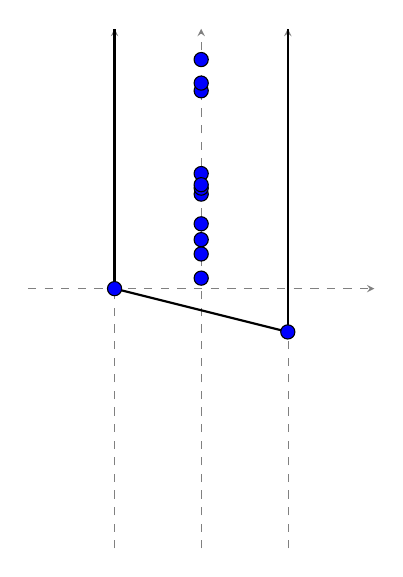
\begin{tikzpicture}[>=stealth, x=1.1cm, y=1.1cm]
            % Dashed lines (axes)
            \draw[help lines, dashed, ->] (-1,0) -- (3,0);
            \draw[help lines, dashed, ->] (0,-3) -- (0,3);
            \draw[help lines, dashed, ->] (1,-3) -- (1,3);
            \draw[help lines, dashed, ->] (2,-3) -- (2,3);
            \draw[thick] (0,0) -- (0,3);
            \draw[thick] (0,0) -- (2, -0.5);
            \draw[thick]  (2,-0.5) -- (2,3);
            \draw[thick]  (2,-0.5) -- (2,3);

            % Points (all with fill=blue and radius=0.09cm)
            \filldraw[fill=blue] (2, -0.5) circle[radius=0.09cm];
            \filldraw[fill=blue] (0, 0) circle[radius=0.09cm]; % Removed duplicate
            \filldraw[fill=blue] (1, 0.12122108098130914) circle[radius=0.09cm];
            \filldraw[fill=blue] (1, 2.28412917072110916) circle[radius=0.09cm];
            \filldraw[fill=blue] (1, 2.3729881287610001) circle[radius=0.09cm];
            \filldraw[fill=blue] (1, 0.4) circle[radius=0.09cm];
            \filldraw[fill=blue] (1, 0.5655158711807637) circle[radius=0.09cm];
            \filldraw[fill=blue] (1, 2.6445016116606668) circle[radius=0.09cm];
            \filldraw[fill=blue] (1, 0.7481703960405396) circle[radius=0.09cm];
            \filldraw[fill=blue] (1, 1.3282219276898275) circle[radius=0.09cm];
            \filldraw[fill=blue] (1, 1.0912647062501184) circle[radius=0.09cm];
            \filldraw[fill=blue] (1, 1.1603772291700336) circle[radius=0.09cm];
            \filldraw[fill=blue] (1, 1.2) circle[radius=0.09cm];
        \end{tikzpicture}~ \caption{A semi-stable lattice}
    \end{minipage} \hspace{3cm} \begin{minipage}{.2\textwidth}
        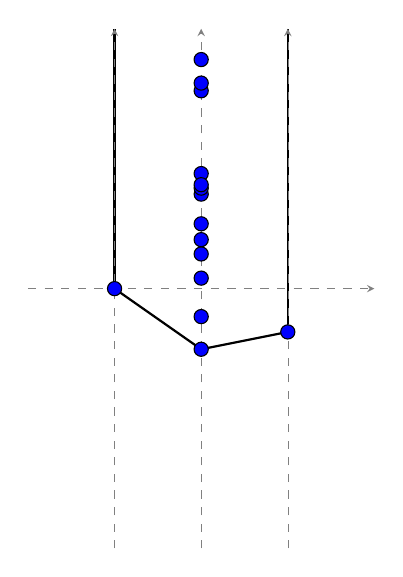
\begin{tikzpicture}[>=stealth, x=1.1cm, y=1.1cm]
            % Dashed lines (axes)
            \draw[help lines, dashed, ->] (-1,0) -- (3,0);
            \draw[thick] (0,0) -- (0,3);
            \draw[thick] (0,0) -- (1, -0.7);
            \draw[thick] (1,-0.7) -- (2,-0.5);
            \draw[thick]  (2,-0.5) -- (2,3);
            \draw[help lines, dashed, ->] (0,-3) -- (0,3);
            \draw[help lines, dashed, ->] (1,-3) -- (1,3);
            \draw[help lines, dashed, ->] (2,-3) -- (2,3);

            % Points (all with fill=blue and radius=0.09cm)
            \filldraw[fill=blue] (2, -0.5) circle[radius=0.09cm];
            \filldraw[fill=blue] (0, 0) circle[radius=0.09cm]; % Removed duplicate
            \filldraw[fill=blue] (1, -0.7) circle[radius=0.09cm];
            \filldraw[fill=blue] (1, -0.3230737092181455) circle[radius=0.09cm];
            \filldraw[fill=blue] (1, 0.12122108098130914) circle[radius=0.09cm];
            \filldraw[fill=blue] (1, 2.28412917072110916) circle[radius=0.09cm];
            \filldraw[fill=blue] (1, 2.3729881287610001) circle[radius=0.09cm];
            \filldraw[fill=blue] (1, 0.4) circle[radius=0.09cm];
            \filldraw[fill=blue] (1, 0.5655158711807637) circle[radius=0.09cm];
            \filldraw[fill=blue] (1, 2.6445016116606668) circle[radius=0.09cm];
            \filldraw[fill=blue] (1, 0.7481703960405396) circle[radius=0.09cm];
            \filldraw[fill=blue] (1, 1.3282219276898275) circle[radius=0.09cm];
            \filldraw[fill=blue] (1, 1.0912647062501184) circle[radius=0.09cm];
            \filldraw[fill=blue] (1, 1.1603772291700336) circle[radius=0.09cm];
            \filldraw[fill=blue] (1, 1.2) circle[radius=0.09cm];
        \end{tikzpicture}~
        \caption{An unstable lattice}
    \end{minipage}
\end{figure}
Visually, a lattice is called \textbf{semi-stable} if it satisfies the other equivalent
conditions:   If $M$ is an arbitrary sublattice of $L$ then $\mu(M) \ge \mu(L)$.
\subsection{Canonical filtration}
Given a lattice $L$ and a sublattice $M \subset L$, the quotient group $L/M$ has the structure of
a lattice. Indeed, consider the exact sequence of lattices
\[0\rightarrow M\rightarrow L\rightarrow L/M\rightarrow 0\]
By tensoring with $\mathbb{R}$ we get a short exact sequence of $\mathbb{R}$-vector subspaces
\[0\rightarrow M_\mathbb{R} \rightarrow L_\mathbb{R} \rightarrow (L/M)_\mathbb{R}\rightarrow 0,\]
which is split. Thus we have the isomorphisms
\[(L/M)_\mathbb{R} \cong L_\mathbb{R}/M_\mathbb{R} \cong M^\perp_\mathbb{R}\]
Therefore, by restricting of the inner product over $L_\mathbb{R}$ to $M^\perp_\mathbb{R}$, we clearly see that
$L/M$ also inherits an inner product. Explicitly, the norm over $L/M$ can be defined by restricting the norm $||\cdot||$ on $L_\mathbb{R}/M_\mathbb{R}$, which is given by
\[||x||:= \inf\{ ||x+m||: m \in M \}\]
\begin{definition}
    Given a lattice $L$ containing a sublattice $M$, then $L/M$ is a lattice. We call this lattice \textbf{quotient lattice}.
\end{definition}
\begin{lemma}\label{volume-of-lattice}\cite[Proposition 4.1]{MR2127941}
    If $L$ is a lattice and $M\subset L$ is a sublattice, we have
    \[\vol(L) = \vol(M)\cdot \vol(L/M)\]
    and if $N$ is any sublattice of $L$ that satisfies $N+M=L$ then
    \[\vol(N) \ge \vol(L/M)\]
\end{lemma}
\begin{proof}
    Assume that $\{m_i\}$ is a basis for the lattice $M$ and $\{e_i\}$ be an orthonormal basis for the vector space
    $M_\mathbb{R}$. Since $M$ is a sublattice of $L$, we can extend the basis $\{m_i\}$ to get a
    basis $\{m_i\} \cup \{n_j\}$ for the lattice $L$. Similarly, we can extend  $\{e_i\}$ to get an orthonormal
    basis $\{e_i\} \cup \{f_j\}$ for the vector space $L_\mathbb{R}$. In particular, we would have
    $\left\langle m_i,f_j \right\rangle =0$ for all $i,j$.
    By definition \ref{covolume-lattice-formula}, we have
    \begin{align*}
        \vol(L) & = \det\begin{bmatrix}
                            \left\langle m_i,e_i\right\rangle  & \left\langle n_j,e_i\right\rangle \\
                            \left\langle m_i,f_J \right\rangle & \left\langle n_j,f_j\right\rangle
                        \end{bmatrix} \\
                & = \det\begin{bmatrix}
                            \left\langle m_i,e_i\right\rangle & \left\langle n_j,e_i\right\rangle \\
                            0                                 & \left\langle n_j,f_j\right\rangle
                        \end{bmatrix}  \\
                & =\vol(M)\cdot \vol(L/M)
    \end{align*}
    Hence we are done. The last inequality follows from the fact that the volume decrease under the orthogonal projection and the observation that
    $N_\mathbb{R} \supset (L/M)_\mathbb{R}$.
\end{proof}
In the canonical plot, the import of lemma \ref{volume-of-lattice} is that the slope of the quotient lattice $L/M$ appears as
the slope of the line segment connecting the points corresponding to the sublattice $M$ and the lattice $L$. This is due to lemma \ref{volume-of-lattice}
\[(\rk(M),\log(\vol(M))+ (\rk(L/M),\log\vol(L/M)))= (\rk(L),\log\vol(L))\]
\begin{figure}[ht]
    \centering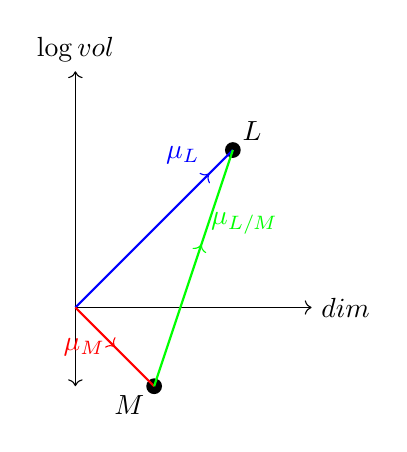
\begin{tikzpicture}
        % Draw axes
        \draw[->] (0,0) -- (3,0) node[right] {$dim$};
        \draw[->] (0,0) -- (0,3) node[above] {$\log vol$};
        \draw[->] (0,0) -- (0,-1);
        % Plot points L and M
        \fill (2,2) circle (0.1) node[above right] {$L$};
        \fill (1,-1) circle (0.1) node[below left] {$M$};

        % Draw lines from origin to L and M with colors
        \draw[thick, blue] (0,0) -- (2,2);
        \draw[thick, red] (0,0) -- (1,-1);

        % Draw line between M and L with color
        \draw[thick, green] (1,-1) -- (2,2);

        % Add mu annotations with matching colors
        \draw[->, blue] (1.5,1.5) -- (1.7,1.7) node[above left] {$\mu_L$};
        \draw[->, red] (0.3,-0.3) -- (0.5,-0.5) node[left] {$\mu_M$};
        \draw[->, green] (1.5,0.5) -- (1.6,0.8) node[above right] {$\mu_{L/M}$};
    \end{tikzpicture}
    \caption{Geometric meaning of slope in canonical plot}
\end{figure}
Given two sublattices $M_1,M_2 \subset L$, if we apply lemma \ref{volume-of-lattice} to the sublattices
$M_1/M_1\cap M_2$ and $M_2/M_1\cap M_2$ in $M_1+M_2/M_1\cap M_2$, we get
\[\vol(M_1/M_1 \cap M_2)\vol(M_2/M_1\cap M_2) \ge \vol(M_1+M_2/M_1\cap M_2)\]
or equivalently
\begin{prop}\label{parallelogram-rule}\cite[Proposition 4.3]{MR2127941}
    Suppose $M_1,M_2$ are sublattices of $L$ then
    \[\log\vol(M_1)+\log\vol(M_2) \ge \log\vol(M_1+M_2)+\log\vol(M_1\cap M_2)\]
\end{prop}


Grayson called this the parallelogram rule, as the geometric meaning of  proposition \ref{parallelogram-rule} is
illustrated in the figure \ref{Grason's parallelogram rule}.
\begin{figure}[hbt!]
    \centering
    \begin{tikzpicture}
        % Coordinates
        \coordinate (A) at (0,0);
        \coordinate (B) at (4,2);
        \coordinate (C) at (6,0);
        \coordinate (D) at (2,-2);
        \coordinate (F) at (4,2.5);
        % Drawing the parallelogram
        \draw (A) -- (B) -- (C) -- (D) -- cycle;

        % Labels
        \node at (A) [above left] {$M_1 \cap M_2$};
        \node at (F) [above] {$M_1$};
        \node at (C) [above right] {$M_1 + M_2$};
        \node at (D) [below] {$M_2$};

        % Points
        \fill[cyan] (A) circle (2pt);
        \fill[cyan] (B) circle (2pt);
        \fill[cyan] (C) circle (2pt);
        \fill[cyan] (D) circle (2pt);
        \fill[cyan] (F) circle (2pt);
    \end{tikzpicture}
    \caption{{Grason's parallelogram  rule}}
    \label{Grason's parallelogram  rule}
\end{figure}
The \textbf{vertices} of the profile are the extremal/lowest points of the plot. Clearly the two points
$(0,0)$ and $(n,\log\vol(L))$ are vertices of the plot of the lattices $L$ with $\rk(L)=n$. The following lemma states the situation for other vertices
of the profile
\begin{lemma}\label{upper-ver}\cite[Lemma 4.4]{MR2127941}
    Suppose that $M_\ast$ is a lattice with with the point $\ell(M_\ast)$ as a vertex of the profile. If $M$ is any other sublattice such that
    $\ell(M)$ is also a vertex of the profile, then we must have either $M \subset M_\ast$ or $M_\ast \subset M$.
\end{lemma}
\begin{figure}[H]
    \centering
    \begin{tikzpicture}
        % Coordinates
        \coordinate (A) at (0,0);
        \coordinate (B) at (4,2);
        \coordinate (C) at (6,0);
        \coordinate (D) at (2,-2);
        \coordinate (F) at (4,2.5);
        \coordinate (E) at (5,-1.5);
        \coordinate (G) at (-1,0);
        \coordinate (H) at (8,-0.5);

        % Drawing the parallelogram
        \draw (A) -- (B) -- (C) -- (D) -- cycle;

        % Labels
        \node at (A) [above left] {$M \cap M_*$};
        \node at (F) [above] {$M$};
        \node at (C) [above right] {$M + M_*$};
        \node at (D) [below] {$M_*$};
        % Points
        \fill[cyan] (A) circle (2pt);
        \fill[cyan] (B) circle (2pt);
        \fill[cyan] (C) circle (2pt);
        \fill[cyan] (D) circle (2pt);
        \fill[cyan] (F) circle (2pt);
        \fill[cyan] (E) circle (2pt);

        % draw additional lines
        \draw[gray] (G) -- (D)-- (E) -- (H);
    \end{tikzpicture}
    \caption{Illustration for lemma \ref{upper-ver}}
    \label{figure33}
\end{figure}
\begin{proof}
    We refer to figure \ref{figure33}. Clearly we can see that the point $\ell(M\cap M_*$) lies somewhere on the left of both
    $\ell(M)$ and $\ell(M_*)$. Similarly, the point $\ell(M+M_*)$ lies somewhere inclusively to the right of $\ell(M)$ and $\ell(M_*)$.
        By the paralellogram rule, the point $ell(M)$ will therefore be above the boundary points
    $\ell(M\cap M_*)$, $\ell(M_*)$ and $\ell(M+M_*)$. If $M$ is also a vertex of the profile, the parallelogram must degenerate. In particular we either have
    $M \cap M*=M$, in which $M\subset M_*$, or $M+M_* = M$, in which $M_* \subset M$.
\end{proof}
An immediate consequence is that
\begin{theorem}\label{filtration}\cite[Theorem 1.18]{MR780079}
    The vertices of the profile of a lattice $L$ are represented by unique sublattices, and they form a chain.
\end{theorem}
For a given lattice $L$, we call the chain of sublattices in theorem \ref{filtration} the \textbf{canonical filtration} of $L$. Assume that the canonical filtration for $L$
is
\[\mathcal{F}: 0 = L_0 \subset L_1 \subset L_2 \subset \cdots \subset L_{k-1} \subset L_k = L \]
then it can be seen from the diagram that
\begin{enumerate}
    \item $L_i/L_{i-1}$ is semi-stable for all $1 \le i \le k$, as the profile of $L_i/L_{i-1}$  is just a straight line segment connecting $\ell(L_{i-1})$ to $\ell(L_i)$.
    \item $\mu(L_i/L_{i-1}) \le \mu(L_{i+1}/L_i)$ for all $1 \le i \le k-1$.
\end{enumerate}
These two conditions is also sufficent for a chain to be a canonical filtration
\begin{theorem}\label{Grayson's criterion}\cite[Corollary 1.30]{MR780079}
    Suppose
    \[\mathcal{F}: 0 = L_0 \subset L_1 \subset L_2 \subset \cdots \subset L_{k-1} \subset L_k = L \]
    is a chain of lattices such that $L_i/L_{i-1}$ is semi-stable and the slope $L_i/L_{i-1}$ is not larger than the slope of $L_{i+1}/L_i$.
    Then this chain is the canonical filtration.
\end{theorem}
\begin{figure}[ht]
    \centering
    \begin{tikzpicture}
        % Coordinates
        \coordinate (A) at (0,0);
        \coordinate (B) at (4,2);
        \coordinate (C) at (6,0);
        \coordinate (D) at (2,-2);
        \coordinate (F) at (4,2.5);
        \coordinate (E) at (5,-1.5);
        \coordinate (G) at (-1,0);
        \coordinate (H) at (8,-0.5);

        % Drawing the parallelogram
        \draw (A) -- (B) -- (C) -- (D) -- cycle;

        % Labels
        \node at (A) [above left] {$M \cap L_{i-1}$};
        \node at (F) [above] {$M$};
        \node at (C) [above right] {$M + L_{i-1}$};
        \node at (D) [below] {$L_{i-1}$};
        \node at (E) [below] {$L_i$};

        % Points
        \fill[cyan] (A) circle (2pt);
        \fill[cyan] (B) circle (2pt);
        \fill[cyan] (C) circle (2pt);
        \fill[cyan] (D) circle (2pt);
        \fill[cyan] (F) circle (2pt);
        \fill[cyan] (E) circle (2pt);

        % draw additional lines
        \draw[gray] (G) -- (D)-- (E) -- (H);
    \end{tikzpicture}
    \caption{Canonical filtration}
    \label{figure34}
\end{figure}
\begin{proof}
    Suppose $M$ to be any other sublattice of $L$. We want to know that $\ell(M)$ lies
    above the plot $P$ of the $\ell(L_i)$. We prove this by induction on the index $i$ such that if $M \subset L_i$
    \begin{itemize}
        \item If $i=1$ then $M\subset L_1$. Since $L_1 $ is semi-stable, we must have $\ell(M)$ lies above the line connecting $(0,0)$ and $\ell(L_1)$. Hence $\ell(M)$ lies above the plot $P$.
        \item Suppose that $M\subset L_i$ for $i>1$. Then $M+L_{i-1} \subset L_i$ contains $L_{i-1}$. Therefore, it corresponds to the point lies above the line connecting $\ell(L_{i-1})$ and $\ell(L_i)$, thus lies above $P$.         By induction, the fact that $(M\cap L_{i-1}) \subset L_{i-1}$ implies $\ell(M\cap L_{i-1})$ lies above the plot $P$. Using the parallelogram rule, the point $\ell(M)$ must then also lie above the plot $P$.
    \end{itemize}
    Thus any chain satisfies the conditions given in the theorem is a canonical filtration.
\end{proof}
\section{$\rho$ semi-stability}
\subsection{$\rho$-definition}
We are now ready to define the $\rho$-definition of semi-stable lattice. Recall that
we define the space of lattices of rank $n$ by $X_n := K \backslash \text{GL}_n(\mathbb{R})$, where $K$ is the orthogonal subgroup
\begin{definition}[\label  = $\rho$-definition]\label{ss2}
    Let $x \in X_n$ be an arbitrary lattice, then the lattice $x$ is called \textbf{$\rho$-semi-stable} if and only if its degree of instability $\deg_{\text{inst}}(x)\ge 0$, where
    \[\deg_{\text{inst}}(x):= \min_{Q \in ParSt, \gamma \in \text{GL}(\mathbb{Q})/Q_i(\mathbb{Q})}\left\langle \rho_Q, H_Q(x\gamma) \right\rangle\]
    and $\text{ParSt}$ stands for the set of standard parabolic subgroup of $\GLn$ as defined in definition \ref{parst}.
\end{definition}
\subsection{Some basic properties}
We first have an elementary lemma and refer to the references for the proof.
\begin{lemma}\label{ss-equiv}\citetext{\citealp[Lemma 2.2.1]{MR3969872}; \citealp[Proposition 4.2.3]{patnaik2025borel}}

    Given $x \in X_n$, then the following are equivalent
    \begin{enumerate}
        \item $\deg_{\text{inst}}(x) \ge 0$.
        \item For every standard parabolic subgroup $P\subset G$ and $\omega \in \widehat{\Delta}_P$ we have \[\left\langle \omega,H_P(x\delta)\right\rangle \ge 0\] for each $\delta \in G(\mathbb{Q})/P(\mathbb{Q})$.
        \item For every maximal parabolic subgroup $Q\subset G$ and $\omega \in \widehat{\Delta}_Q$ we have \[\left\langle \omega,H_Q(x\delta)\right\rangle \ge 0\] for each $\delta \in G(\mathbb{Q})/Q(\mathbb{Q})$.
    \end{enumerate}
\end{lemma}
\subsection{Check for semi-stability}\label{semi-stable-verified}
From lemma \ref{ss-equiv}, to check whether $x \in G$ is semi-stable, we just need to verify whether $$\left\langle \omega,H_Q(x\delta)\right\rangle \ge 0.$$
for $\omega \in \widehat{\Delta}_Q$ and $Q \subset G$ a standard maximal parabolic subgroup.
From lemma \ref{coeff-H(J)}
\[H_B = H_Q+H(Q)_{\ast B}\]
where $H_Q$ is a scalar multiple of $\lambda_i^\vee$ for $Q = Q_i$ and $H(Q)_{\ast B}$ is a linear combination of $\alpha_j^\vee$ for $ j \ne i$.
On the other hand, since $Q$ is a maximal standard parabolic subgroup of $G$,
$\omega$ is proportional to $\lambda_i.$ Thus $$\left\langle \omega H(Q)_{\ast B}(x\gamma)\right\rangle =0.$$ In particular, we can replace $H_Q$ by $H_B$ in verifying semi-stability.
Write
\[ x\gamma = kan, \quad k \in K, a \in A, n \in N,\]
as in Iwasawa decomposition, and set $H_B(x) = H$ where $H = \exp(a)$. In particular, if
\[a = \begin{bmatrix}
        a_1    & 0      & \ldots & 0      \\
        0      & a_2    & \ldots & 0      \\
        \vdots & \vdots & \vdots & \vdots \\
        0      & 0      & \ldots & a_n
    \end{bmatrix}\]
then
\begin{equation}
    \left\langle \rho_{Q_i}, H_B(x\gamma) \right\rangle = \dfrac{n}{2}\log(a_1a_2\ldots a_i) \label{volume - H_P}
\end{equation}
Thus, to check for the semi-stability of a lattice $x$, we just need to look at the
$A$-coordinate of $x\gamma$ for every $\gamma \in G(\mathbb{Q})/Q_i(\mathbb{Q})$, and verify whether the following system holds
\begin{align*}
    \begin{cases}
        a_1 \ge 1   \\
        a_1a_2\ge 1 \\
        \ldots      \\
        a_1a_2\ldots a_n \ge 1
    \end{cases}
\end{align*}
\section{Canonical pair}
Consider a pair $(P,\delta)$ of a standard parabolic subgroup $P \subsetneq G$ and $\delta \in G(\mathbb{Q})/P(\mathbb{Q})$. Such a pair is called \textbf{destabilizing} for $x$ if
\[\left\langle \rho_P, H_P(x\delta)\right\rangle = \deg_{\text{inst}}(x)\]
Such a pair is called \textbf{extremal} for $x$ if for any standard parabolic $Q \subset P$ such that
\[\left\langle \rho_Q, H_Q(x\delta)\right\rangle = \left\langle \rho_P, H_P(x\delta)\right\rangle\]
then $Q=P$.
\begin{definition}
    A pair $(P,\delta)$ that is both \textit{destabilizing} and \textit{extremal} for $x$ is called a \textbf{canonical pair} for $x$.
\end{definition}
A canonical pair for $x$, if exists, will be denoted by $\cpx:=(P,\delta)$. A priori, it is not clear whether $\cpx$ exists or not.
We will show that it is in fact equivalent to the notion of canonical filtration introduced in the previous sections, and deduce that
$\cpx$ must exist and it is unique.

We obtain the following lemma as a consequence of the definition of canonical pair
\begin{lemma}\label{canonical-pair}\citetext{\citealp[Lemma 2.3.2]{MR3969872}; \citealp[Lemma 4.2.5]{patnaik2025borel}}
    Let $x \in X_n$  and $(P,\delta)$ be a pair with $P \subsetneq G$ be standard parabolic subgroup and
    $\delta \in G(\mathbb{Q})/P(\mathbb{Q})$. Then
    \begin{enumerate}
        \item If $(P,\delta)$ is destabilizing for $x$, then $\deg_{inst}^P(x\delta) \ge 0$. \label{destabilizing}
        \item If $(P,\delta) $ is extremal for $x$, then $\left\langle \alpha, H_P(x\delta)\right\rangle < 0$ for any $\alpha \in \Delta_P$.\label{extremal}
    \end{enumerate}
\end{lemma}
\begin{proof}
    For the first part, let $Q \subset P$ be any standard parabolic, then
    \[\rho_Q = \rho_P + \rho_Q^P\]
    Thus, for any $\eta \in P(\mathbb{Q})/Q(\mathbb{Q})$
    \begin{align*}
        \left\langle \rho_Q^P,H_Q(x\gamma\eta)\right\rangle & = \left\langle\rho_Q,H_Q(x\gamma\eta)\right\rangle - \left\langle\rho_P,H_P(x\gamma\eta)\right\rangle \\                                                 & = \left\langle\rho_Q,H_Q(x\gamma\eta)\right\rangle -\deg_{inst}(x) \ge 0
    \end{align*}
    For the second part, we can pick a standard parabolic $Q \subset G$ containing $P$ such that $P$ is maximal in $Q$. In particular, we have
    $\Delta^{Q}_P = \{\alpha\}$. Then
    \begin{align*}
        \left\langle\rho_P^Q,H_P(x\delta)\right\rangle & = \left\langle\rho_P,H_P(x\gamma)\right\rangle - \left\langle\rho_Q,H_Q(x\gamma\eta)\right\rangle \\
                                                       & = \deg_{inst}(x) - \left\langle\rho_Q,H_Q(x\gamma\eta)\right\rangle <0
    \end{align*}
    Since $\rho_P^Q$ and $\alpha$ are proportional by a positive number, the result follows immediately.\end{proof}

\chapter{Equivalence between semistability and $\rho$-semistability}
\section{The equivalent between definitions of semi-stable lattices}
So far we have two distinct definitions of semi-stability. The following theorem asserts that they are equivalent:
\begin{prop}\label{semi-stable-equiv}
    Let $x \in X_n = K \backslash \text{GL}_n(\mathbb{R})$ - the space of unit lattice. Then $x$ is semi-stable if one of the following equaivalent
    conditions holds
    \begin{enumerate}
        \item The bottom of the profile of $x$ is a line connect solely two points: the origin and $(n,0)$.
        \item The degree of instability of $x$ is nonnegative, namely, $\deg_{inst}(x) \ge 0$.
    \end{enumerate}
\end{prop}
\begin{proof}
    \hfill \\
    If we can prove there is a correspondence between
    $\gamma \in \text{GL}_n(\mathbb{Q})/Q_i(\mathbb{Q})$ and a sublattice of rank $i$ of $x$, then we are done.
    We first need a slight reduction - we identified the quotient $\text{GL}_n(\mathbb{Q})/Q_i(\mathbb{Q})$ with
    the quotient $\text{GL}_n(\mathbb{Z})/(Q_i(\mathbb{Q}) \cap \text{GL}_n(\mathbb{Z})) $. Now let $x$ be an arbitrary lattice of rank $n$.

    We will first show the following correspondence
    \[ \text{GL}_n(\mathbb{Z})/(Q_i(\mathbb{Q}) \cap \text{GL}_n(\mathbb{Z})) \longleftrightarrow \left\lbrace \text{ sublattice of rank $i$ of $\mathbb{Z}^n$}\right\rbrace\]
    We define the map from the collection of sublattices of rank $i$ to the cosets space as follows: For any sublattice $M \subset \mathbb{Z}^n$, there exists
    a basis of $M$, denoted by
    \[\left\lbrace v_1,v_2,\ldots, v_i \right\rbrace \]
    we can extend this basis to get a basis of $\mathbb{Z}^n$
    \[\mathfrak{B'} = \left\lbrace v_1,v_2,\ldots, v_n \right\rbrace \]
    Clearly in $\mathbb{Z}^n$ we have the standard basis $\mathfrak{B} = \left\lbrace e_1,e_2,\ldots,e_n\right\rbrace $. Clearly there
    exists a map $\gamma \in \glnz$ such that
    \[\gamma \cdot e_k = v_k \quad \forall k = 1,2,\ldots, n\]
    So we define the map
    \begin{align*}
        \varphi \colon \left\lbrace\text{sublattices of rank $i$ of $\mathbb{Z}^n$}\right\rbrace & \to \text{GL}_n(\mathbb{Z})/(Q_i(\mathbb{Q}) \cap \text{GL}_n(\mathbb{Z})) \\
        M                                                                                        & \mapsto [\gamma]
    \end{align*}
    where $[\gamma]$ denoted the equaivalent class of $\gamma$ in the quotient space. This is a well-defined map. Indeed, Assume that we extend
    the basis $\mathfrak{B'}$ in a different way to get the basis
    \[ \mathfrak{B}_1 = \left\lbrace v_1,\ldots, v_k, v'_{k+1},\ldots,v'_n \right\rbrace\]
    As above, there also exists $\gamma' \in \glnz$ such that
    \[\gamma' e_k = v_k \quad \forall k \le i, \quad \text{ and } \quad \gamma'e_k = v'_k \quad \forall k > i\]
    But this implies that
    \[(\gamma^{-1})\gamma ' \cdot e_k = \gamma^{-1} v_k = e_k \quad \forall k \le i\]
    So in particular, we have $[\gamma] = [\gamma']$. The inverse map is given by
    \[[\gamma] \mapsto \bigoplus_{k=1}^i\mathbb{Z} (\gamma \cdot e_i) = M\]
    This generalizes in the obvious way for lattice $x = g\mathbb{Z}^n$ for some $g \in \text{GL}_n(\mathbb{R})$. Indeed, we just define
    the map
    \begin{align*}
        \phi_g \colon \left\lbrace\text{sublattices of rank $i$ of $g\mathbb{Z}^n$}\right\rbrace & \to \text{GL}_n(\mathbb{Z})/(Q_i(\mathbb{Q}) \cap \text{GL}_n(\mathbb{Z})) \\
        M_g = gM = g \bigoplus_{k=1}^i  \mathbb{Z}v_i                                            & \mapsto [\gamma]
    \end{align*}
    where $\gamma e_k = v_k$ in $\mathbb{Z}^n$ for all $ k \le i$ and $\phi_g^{-1}([\gamma]) = g \bigoplus_{k=1}^i  \mathbb{Z}(\gamma \cdot e_i)$.
\end{proof}\todo{Check the map in the generalization carefully }
\section{Canonical pair and Canonical filtration}
We can further prove that, the equivalence between different notions of semistability
comes from the equivalence between the notion of canonical pair and the bottom of the
profile of a lattice - the canonical filtration. The main result is the following proposition
\begin{prop}\label{cp-equiv}
    Given an $x \in X_n = K\backslash G$. Then $(P,\delta)$ is the canonical pair for $x$ if and only if $P$
    is the stabilizer of the canonical filtration for the lattice $L_x = x\mathbb{Z}^n$.
\end{prop}
Recall that, from theorem \ref{Grayson's criterion} and lemma \ref{canonical-pair}, both canonical
pair and canonical filtration are characterized by two conditions. We will show that these two conditions are equivalent.
Throughout this section, we fix an $x \in X_n$ and the corresponding lattice $L_x= x\mathbb{Z}^n$.
\begin{lemma}\label{increasing-slope}
    The the following conditions are equivalent
    \begin{enumerate}
        \item  $\left\langle \alpha, H_P(x\delta)\right\rangle <0$ for any $\alpha \in \Delta_P$ and for some $\delta \in G_\mathbb{Q}/P_\mathbb{Q}$.
        \item $L_x$ has a chain of vector spaces
              \[\mathcal{F}: 0 = L_0 \subset M_1 \subset M_2 \subset \cdots \subset M_{k-1} \subset M_k = L_x \]
              such that $\mu(M_i/M_{i-1}) <\mu(M_{i+1}/M_i)$ for all $i$. We also attach to the flag
              \[\mathcal{F}\otimes \mathbb{R} \colon L_0 \subset M_1 \otimes \mathbb{R} \subset M_2\otimes \mathbb{R} \subset \cdots \subset M_{k-1}\otimes \mathbb{R} \subset M_k\otimes \mathbb{R} =  \mathbb{R}^n \]
              a rational standard parabolic subgroup $P_\mathbb{Q}$.
    \end{enumerate}
\end{lemma}
\begin{proof}

    We first prove (1) implies (2). Assume that $(P,\delta)$ is the canonical pair for $x$ and
    \[a(x\delta) = \begin{bmatrix}
            a_1    & 0      & \ldots & 0      \\
            0      & a_2    & \ldots & 0      \\
            \vdots & \vdots & \vdots & \vdots \\
            0      & 0      & \ldots & a_n
        \end{bmatrix}\]
    in the Iwasawa decomposition of $x\delta$. We further assume that the standard parabolic
    $P$ in the canonical pair is of type $(n_1,\ldots, n_k)$. Let
    \[d_i = n_1+n_2+\ldots +n_k\]
    Then from the chain of standard lattice
    \[0 \subset \mathbb{Z}^{d_1} \subset \mathbb{Z}^{d_2} \subset \cdots \subset \mathbb{Z}^{d_k}\]
    we obtain a chain of sublattices of $L_x$ as follows
    \[0 \subset M_1 \subset M_2 \subset \cdots \subset M_k\]
    where $$M_i := \bigoplus_{m=1}^{d_i}\mathbb{Z}x\delta \cdot e_m$$.

    Note that for $M_k = x\delta\mathbb{Z}^{d_k} = x\mathbb{Z}^n = L_x$.

    since the volume depend solely on the $A$-coordinate in the Iwasawa decomposition.
    In this way, it is immediate that the volume of the sublattice $M_i$ is
    \[\vol(M_i) = a_1a_2\cdots a_i,\]
    \begin{figure}[hbt]
        \centering
        \begin{tikzpicture}
            % Coordinates
            \coordinate (D) at (2,-2);
            \coordinate (F) at (4,2.5);
            \coordinate (E) at (8,-2);
            \coordinate (G) at (-1,0);
            \coordinate (H) at (12,0);
            % Labels
            \node at (G) [below] {$\cdots$};
            \node at (D) [below] {$M_i(d_i,\log(a_1\cdots a_{d_i}))$};
            \node at (E) [below ] {$M_{i+1}(d_{i+1}\log(a_1\cdots a_{d_{i+1}}))$};
            \node at (H) [below ] {$\cdots$};
            % Points
            \fill[cyan] (E) circle (2pt);
            \fill[cyan] (D) circle (2pt);
            \fill[cyan] (G) circle (2pt);
            \fill[cyan] (H) circle (2pt);

            % draw additional lines
            \draw[gray] (G) -- (D)-- (E) -- (H);
        \end{tikzpicture}
        \caption{}
        \label{figureproof}
    \end{figure}



    We will show that
    \[H_P(x\delta ) =m_1\lambda^\vee_{d_1}+m_2\lambda^\vee_{d_2}+\ldots+m_k\lambda^\vee_{d_k}\]
    where
    \[m_i = \dfrac{\log(a_{d_{i-1}}\cdots a_{d_i})}{n_i}-\dfrac{\log(a_{d_i+1}\cdots a_{d_{i+1}})}{n_{i+1}}\]
    If we can prove this, we are done, as
    \[ \mu(M_i/M_{i-1})-\mu(M_{i+1}/M_i)= m_i =\left\langle\alpha_{d_i},H_P(x\delta) \right\rangle < 0\]
    Hence we recover the second condition in Grayson's criterion, namely, $\mu(M_i/M_{i-1}) \le \mu(M_{i+1}/M_i)$ for all $1 \le i \le k-1$.

    To prove this, we first note that
    \begin{align*}
        H_B(x\delta) & =  \log(a_1)\alpha_i^\vee+\log(a_1a_2)\alpha_2^\vee+\ldots \log(a_1a_2\cdots a_{n-1})\alpha_{n-1}^\vee             \\
                     & = \log\left(\dfrac{a_1}{a_2}\right)\lambda_1^\vee+\ldots + \log\left(\dfrac{a_{n-1}}{a_n}\right)\lambda_{n-1}^\vee
    \end{align*}
    To compute $H_P(x\delta)$, we will use the Lemma \ref{H_P-decomp} to get
    \[H_B =H_P + H_{\star B}\]
    and Lemma \ref{coeff-H(J)} to compute $H_{\star B}$ explicitly. Since $P$ is a standard parabolic
    subgroup, we have $P=P_J$ and thus
    \[H_{\star B}(x\delta) = \sum_{i \notin J} \log\left(\dfrac{a_i}{a_{i+1}}\right)\lambda_{i,J}^\vee\]
    We want to write $\lambda_{i,J}^\vee$ as linear combination of $\alpha_j^\vee$'s. To do this, we use
    the theorem \ref{cartaininverse}.

    Note that we can write $H_P(x\delta)$ in two ways
    \begin{align*}
        H_P(x\delta) & = H_B(x\delta) - H_{\star B}(x\delta)                                     \\
                     & = \sum_{j=1}^{n-1}t_j\alpha_j^\vee                                        \\
                     & =m_1\lambda^\vee_{d_1}+m_2\lambda^\vee_{d_2}+\ldots+m_k\lambda^\vee_{d_k}
    \end{align*}
    Then by \ref{weight-root-comb}, we must have
    \[m_i = 2t_{d_i}-t_{d_{i}-1}+t_{d_i+1}\]
    for $1<i<k$. To compute $t_{d_i}$, we find the coefficient of $\alpha_{d_i}^\vee$. But this
    is just the coefficient of $\alpha_{d_i}^\vee$ in the linear combination of $H_B(x\delta)$. Thus
    \[t_{d_i} = \log(a_1\cdots a_{d_i})  \]
    The value of $t_{d_i-1}$ and $t_{d_i+1}$ is slightly more complicated. For $t_{d_i-1}$, it is the difference between
    the coefficient of $\alpha_{d_i-1}^\vee$ in $H_B(x\delta)$ and that of $\alpha_{d_i-1}^\vee$ in $H_{\star B}(x\delta)$.
    By lemma \ref{cartaininverse}, we have
    \begin{align*}
        \sum_{s=p}^q\log\left(\dfrac{a_s}{a_{s+1}}\right)\lambda^\vee_s
         & =\begin{bmatrix}
                \log\left(\dfrac{a_p}{a_{p+1}}\right) & \cdots & \log\left(\dfrac{a_q}{a_{q+1}}\right)
            \end{bmatrix}
        \begin{bmatrix}
            \lambda_p^\vee \\
            \vdots         \\
            \lambda_q^\vee
        \end{bmatrix}                                                                                                                                     \\
         & =\begin{bmatrix}
                \log\left(\dfrac{a_p}{a_{p+1}}\right) & \cdots & \log\left(\dfrac{a_q}{a_{q+1}}\right)
            \end{bmatrix}  A^{-1} \begin{bmatrix}
                                      \lambda_p^\vee \\
                                      \vdots         \\
                                      \lambda_q^\vee
                                  \end{bmatrix}
    \end{align*}
    So the coefficient of $\alpha_{d_i-1}^\vee$ in $H_{\star B} (x\delta)$ is
    \[\sum_{u=1}^{n_i-1}\log\left(\dfrac{a_{d_{i-1}+u}}{a_{d_{i-1}+u+1}}\right)\left(\min\{u,n_i-1\}-\dfrac{u(n_i-1)}{n_i}\right)=\sum_{u=1}^{n_i-1}\log\left(\dfrac{a_{d_{i-1}+u}}{a_{d_{i-1}+u+1}}\right)\dfrac{u}{n_i}\]
    Argue similarly, we can also find the value of $t_{d_i+1}$. Overall, we have
    \begin{align*}
        \begin{cases}
            \displaystyle  t_{d_i-1} = \log(a_1\cdots a_{d_i-1})-\sum_{u=1}^{n_i-1}\log\left(\dfrac{a_{d_{i-1}+u}}{a_{d_{i-1}+u+1}}\right)\dfrac{u}{n_i}                  \\
            \displaystyle t_{d_i+1}= \log(a_1\cdots a_{d_i+1})-\sum_{u=1}^{n_{i+1}-1}\log\left(\dfrac{a_{d_{i}+u}}{a_{d_{i}+u+1}}\right)\left(1-\dfrac{u}{n_{i+1}}\right) \\
        \end{cases}
    \end{align*}
    which simplify to $m_i = \dfrac{\log(a_{d_{i-1}}\cdots a_{d_i})}{n_i}-\dfrac{\log(a_{d_i+1}\cdots a_{d_{i+1}})}{n_{i+1}}$ as desired.
    The cases $i=1,k$  can be verified similarly.

    Conversely, assume that we have a a chain
    \[\mathcal{F}: 0 = L_0 \subset M_1 \subset M_2 \subset \cdots \subset M_{k-1} \subset M_k = L_x \]
    Then multiplying by $x^{-1}$ on the left gives a chain of lattices in $\mathbb{Z}^n$.
    \[\mathcal{F}: 0 = L_0 \subset N_1 \subset N_2 \subset \cdots \subset N_{k-1} \subset N_k ^n= \mathbb{Z} \]
    where $N_i:= x^{-1}M_i$. Let us denote $n_i:=\rk(N_i)$. Then there exists an ordered
    basis for the standard lattice $\mathbb{Z}^n$
    \[\mathcal{B} = \left\lbrace v_1,v_2,\ldots, v_n \right\rbrace\]
    such that $\{v_1,\ldots,v_{n_i}\}$ is the basis for the lattice $N_i$. We clearly can find an element
    $\delta \in \glnz$ such that $\delta\cdot v_i = e_i$. Repeat the argument in Theorem \ref{semi-stable-equiv}, we can see that
    $\delta\eta$ stabilizes the flag $\mathcal{F}$. So it does not change anything if we consider the coset $\delta P_\mathbb{Q}$.
    Consider the element $x\delta$ for $\delta \in G_\mathbb{Q}/P_\mathbb{Q}$ and do the same computation for
    $x\delta$ as in the $1 \Rightarrow 2$ part, we can see that
    \[0 > \mu(M_i/M_{i-1})-\mu(M_{i+1}/M_i)= m_i =\left\langle\alpha_{d_i},H_P(x\delta) \right\rangle\]
    Thus the lemma is proved.
\end{proof}
\begin{remark}
    From the proof the lemma \ref{increasing-slope}, we explicitly construct an equivalence
    \[xG_\mathbb{Q}/P_\mathbb{Q} \longleftrightarrow \{\mbox{ flag of sublattices of $x\mathbb{Z}^n$ of the same type of partition type of $P$}\}\]

\end{remark}
\begin{lemma}\label{ss-slope}
    Fixed the notations as in lemma \ref{increasing-slope}, the following conditions are equivalent
    \begin{enumerate}
        \item $M_i/M_{i-1}$ is semistable for all $i$, where the flag
              \[\mathcal{F}: 0  \subset M_1 \subset M_2 \subset \cdots \subset M_{k-1} \subset M_k = L_x \]
              corresponds to $x\delta$.
        \item $x\delta$ is $P-$semistability for some $\delta \in G_\mathbb{Q}/P_\mathbb{Q}$.
    \end{enumerate}
\end{lemma}
\begin{proof}
    \hfill \\
    We prove $1 \Rightarrow 2$ by contradiction. Assume not, then there exists a maximal
    parabolic subgroup $Q \subset P$ and an $\eta \in P/Q$ such that
    \[\left\langle \rho_Q^P, H_Q(x\delta\eta) \right\rangle < 0\]
    by lemma \ref{ss-equiv}. We assume that $P$ is a standard parabolic subgroup of type $(n_1,n_2,\ldots,n_k)$. Then
    Q must be of the type $(n_1,\ldots, n_{i,1},n_{i,2},\ldots,n_k)$ where $n_{i,1}+n_{i,2} = n_i$
    for some $1 \le i \le k$.  Argue as in lemma \ref{increasing-slope}, we obtain a chain of sublattices of $L_x$
    \[0 \subset M_{1} \subset \cdots M_{{i-1}} \subset M'\subset M_{{i+1}} \subset \cdots \subset M_{k} = L_x\]
    where $\rk(M_j)=d_j$ for $j \ne i$ and $\rk(M') = d_{i-1}+n_{i,1} =r$.

    Using the same computation as in lemma \ref{increasing-slope}, it can be seen that
    \[0 > \left\langle\rho_Q^P, H_Q(x\delta\eta)\right\rangle = c \left\langle \alpha_r,H_Q(x\delta\eta) \right\rangle= c\cdot\left(\mu(M'/M_{i-1})-\mu(M_{i+1}/M')\right) \]
    In particular
    \[\mu(M'/M_{i-1})-\mu(M_{i+1}/M') < 0 \Leftrightarrow \mu(M'/M_{i-1})<\mu(M_{i+1}/M')\]
    But this contradicts the fact that $M_i/M_{i-1}$ is a semistable for all $i$, i.e.
    there are no sublattices $M'$ such that $\ell(M')$ lies below the line connectings
    $\ell(M_i)$ and $\ell(M_{i-1})$ for all $i$.
    \begin{figure}[hbt]
        \centering
        \begin{tikzpicture}
            % Coordinates
            \coordinate (D) at (2,-2);
            \coordinate (F) at (4,2.5);
            \coordinate (A) at (6,-4);
            \coordinate (E) at (8,-3);
            \coordinate (G) at (-1,0);
            \coordinate (H) at (12,-1);
            % Labels
            \node at (A) [below] {$\ell(M')$};
            \node at (D) [below] {$\ell(M_{i-1})$};
            \node at (E) [below ] {$\ell(M_{i})$};
            % Points
            \fill[cyan] (E) circle (2pt);
            \fill[cyan] (D) circle (2pt);
            \fill[cyan] (A) circle (2pt);
            \fill[cyan] (H) circle (2pt);
            \fill [cyan] (G) circle (2pt);
            % draw additional lines
            \draw[thick,black] (G) -- (D)-- (E) -- (H);
            \draw[red] (D) -- (A) -- (E);
        \end{tikzpicture}
        \caption{}
        \label{figureproof}
    \end{figure}

    Conversely, to prove $2 \Rightarrow 1$, we also prove by contradiction.
    Assume that $M_i/M_{i-1}$ is unstable for some index $i$. Then there exists
    a flag
    \[ 0 \subset M^\ast \subset M_i/M_{i-1}\]
    such that $\mu(M^\ast) <\mu(M_i/M_{i-1})$. Let $M':= M^\ast \oplus M_{i-1}$, then
    $M'$ is a sublattice of $M_i$ containing $M_{i-1}$ such that
    \[\mu(M'/M_{i-1}) < \mu (M_i/M_{i-1}) = \dfrac{rk (M'/M_{i-1})}{\rk(M_i/M_{i-1})}\mu(M'/M_{i-1})+\dfrac{rk (M_i/M')}{\rk(M_i/M_{i-1})}\mu(M_i/M') \]
    which implies that
    \[\mu(M'/M_{i-1})<\mu(M_i/M')\]
    Since the chain
    \[0 \subset M_{1} \subset \cdots M_{{i-1}} \subset M'\subset M_{{i+1}} \subset \cdots \subset M_{k} = L_x\]
    is a refinement of the flag $\mathcal{F}$, this gives rise to a pair $(Q,\delta')$ where $Q\subset P$
    is a maximal standard parabolic subgroup of $P$ and $\delta'P=\delta P$. But then again we have
    \[ \left\langle\rho_Q^P, H_Q(x\delta\eta)\right\rangle = c \left\langle \alpha_r,H_Q(x\delta\eta) \right\rangle= c\cdot\left(\mu(M'/M_{i-1})-\mu(M_{i+1}/M')\right)<0 \]
    which is a contradiction.
\end{proof}
Combinining Lemmas \ref{ss-slope} and \ref{increasing-slope}, we get a proof
for proposotion \ref{cp-equiv} as follows
\begin{proof}
    Assume that $(P,\delta)$ is a canonical pair for $x$, then there exists a
    flag
    \[\mathcal{F}: 0 = L_0 \subset M_1 \subset M_2 \subset \cdots \subset M_{k-1} \subset M_k = L_x \]
    that corresponds to $x\delta$ and admits $P_\mathbb{Q}$ as its stabilizer. Lemmas \ref{increasing-slope}
    and \ref{ss-slope} guarantees that this flag satisfies two condition in Grayson's criterion \ref{Grayson's criterion}, thus
    $\mathcal{F}$ is the canonical filtration. Conversely, let $\mathcal{F}$ be the canonical
    filtration for $x$ and denote $Q$ the stabilizer of $\mathcal{F}$. If $(P,\delta)$ is the canonical pair, it also gives
    rise to a canonical flag $\mathcal{F'}$. Theorem \ref{filtration} ensures that the canonical filtration is unique, thus
    $\mathcal{F} \equiv \mathcal{F'}$. Consenquently, we must have $Q=P$.
\end{proof}
\begin{remark}
    The construction above also shows that the canonical pair, must be unique and determined by the canonical filtration.
\end{remark}
\bibliographystyle{plainnat}
\bibliography{refs}

\end{document}
